%!TEX root = ../thesis.tex
%*******************************************************************************
%****************************** Fifth Chapter **********************************
%*******************************************************************************
\chapter{High-Resolution CMB Bispectrum Estimator}

% **************************** Define Graphics Path **************************
\ifpdf
    \graphicspath{{Chapter5/Figs/Raster/}{Chapter5/Figs/PDF/}{Chapter5/Figs/}}
\else
    \graphicspath{{Chapter5/Figs/Vector/}{Chapter5/Figs/}}
\fi

Despite their major role in constraining a wide range of inflation models, there are only a few implementations of the CMB bispectrum estimator due to computational challenges. The Planck collaboration mainly utilised three independent approaches for their bispectrum analysis \cite{PlanckCollaboration2015,PlanckCollaboration2018}: KSW \cite{Komatsu2005}, Binned \cite{Bucher2010}, and Modal \cite{Fergusson2012}. Standard bispectrum templates for Local, Equilateral and Orthogonal shapes have been constrained using all three methods independently, while other more specific ones were covered by only a subset of them.

Some of the most challenging models to handle are those with oscillatory behaviour. Numerous theoretically well-motivated models fall into this category. Feature models, as discussed in the previous chapter, often predict linearly spaced oscillations in the bispectrum. Resonance models such as Axion monodromy, ones with varying speed of sound, ... all produce log-spaced oscillations modulated with various envelopes. (CHECK! NBD, DBI? PUT LOTS OF REFS HERE). Constraining such models are difficult since wobbles in the bispectra degrade numerical stability of the integrals involved.

Several simple models with oscillations have been studied in the latest Planck analysis using Modal and some specific KSW-type estimators introduced in \cite{Munchmeyer2014}. Modal estimator covers wide range of oscillatory models, with and without envelopes, thanks to versatility of its mode expansion. It is however difficult to constrain models with high-frequency oscillations using generic mode functions. Modal code allows choosing a more tailored set of modes for this purpose, but the fact that there are \textit{two} independent sets of mode functions - primordial and late-time - complicates targeted analyses. For each specific selection of mode functions in primordial `$k$' domain, a suitable choice of basis has to be made in late-time `$l$' space. Rapidly oscillating signals may also get lost during the projection from one to the other and cause some numerical issues.

On the other hand, adapted KSW-type estimators (\cite{Munchmeyer2014}, PUT ONE MORE FOR SINLOG!) may probe models with arbitrarily fast modulations in their bispectra. They exploit separability of specific oscillatory templates to obtain accurate constraints in model-by-model basis. However, this method is not applicable for any model with slightly more complicated bispectra. Even in cases where some clever mathematical trick enables calculation, it may not be always straightforward to modify the code accordingly. This was one of the main motivations behind this research project; can we have a bispectrum estimator which has the efficiency and versatility of Modal, but also benefits from the flexibility of KSW formalism for targeted analysis?

We developed a novel CMB bispectrum estimation pipeline CMB-BEst. \footnote{Short for \underline{CMB} \underline{B}ispectrum \underline{Est}imator. The goal of CMB-BEst is to be the best bispectrum estimator with wide applications and great precision.} CMB-BEst has two main strengths over former methods. First of all, it is implemented for completely general basis sets, which allows broad analyses on inflationary models. In fact, the conventional KSW estimator is equivalent to a specific choice of basis in \textit{CMB-BEst}. CMB-BEst can cover any model KSW estimator can, and does more; it can simultaneously constrain general bispectrum shapes through primordial mode expansion, just like Modal.

Secondly, CMB-BEst is designed to be able to handle complex and highly oscillatory signals. It does not require a separate set of basis functions for late-time $l$ space, in contrary to Modal. More diverse and specialised choice of basis can therefore be made. The code will be used on numerous inflation models with complex oscillations yet to be investigated due to lack of resolution from previous methods. Potential choices of targeted basis for this purpose will be discussed in Section \ref{section:basis_functions}.

Every good thing comes at a price. For CMB-BEst, the price is computational cost. Combining the best of Modal and KSW estimators, CMB-BEst's formalism is more numerically demanding than both of them. Na\"ively speaking, running CMB-BEst for one set of basis functions is equivalent to computing thousands of KSW estimators put together. It is prohibitively expensive unless properly and thoroughly optimised.

We invested considerable amount of time and effort on optimising the code. Separable mode expansions and subsequent algorithm design were studied in detail for maximal reduction in computational complexity. We also made full use of parallelisation techniques to exploit modern computing architecture. Improving data locality for efficient memory access yielded an order of magnitude speed-up. We illustrate our optimisation procedure in Section \ref{section:implementation}.

The code was then tested thoroughly both internally and against Planck analysis. We used CMB maps and simulations from the Planck satellite experiment and checked that \textit{CMB-BEst} agrees with previous routines map-by-map for various bispectrum templates. Different choices of basis functions within \textit{CMB-BEst} also yielded consistent results. We dedicate Section \ref{section:validation} to present the outcome of these consistency checks.

Lastly, we present some applications of the code which serves as a proof of concept. In particular, we connect CMB-BEst to \textsc{Primodal}, an efficient numerical code for computing bispectra of primordial perturbations from a given single field model \cite{Clarke2021}. \textsc{Primodal} uses separable modes for its computation, which enables template-free, direct model-to-constraint analysis when combined with CMB-BEst appropriately. Section \ref{section:proof_of_concept} highlights some results from the combined pipeline. We also identify rooms for improvement and discuss future research direction.

Upcoming surveys will provide major improvements to constraints on primordial non-Gaussianity. Inflationary models with oscillations would also greatly benefit from the enhanced sensitivity, as we discussed in the previous chapter. It is therefore crucial to have a robust and flexible bispectrum estimation routine ready for the future surveys, especially the one which can handle high-frequency oscillations. Having another code independent from the existing ones would also be greatly beneficial for cross validation. We expect CMB-BEst to fill this role in near future.


\section{Formalism}

\subsection{CMB-BEst formalism}
Recall that the optimal CMB bispectrum estimator for a given template can be written as
\begin{align}
	\hat{f}_{NL} = \frac{1}{N} \sum_{l_j,m_j} \frac{\mathcal{G}^{l_1 l_2 l_3}_{m_1 m_2 m_3} b_{l_1 l_2 l_3}}{C_{l_1} C_{l_2} C_{l_3}} \left[ a_{l_1 m_1} a_{l_2 m_2} a_{l_3 m_3} - \left( \left< a^G_{l_1 m_1} a^G_{l_2 m_2} \right> a_{l_3 m_3} + \text{2\ cyc.} \right)  \right].		\label{eqn:bispectrum_estimator_standard}
\end{align}
Here we omit superscripts $X$ for temperature and polarisation for notational convenience. Even though the formalism in this section will be presented for CMB temperature data only, the method is general and can easily be extended to include polarisation. For estimation of the full covariance matrix $C_{lm,l'm'}$ needed for the linear term, we use ensemble average from Gaussian simulations, as denoted by superscripts $G$ and the bracket $\left<\cdot\right>$.

The normalisation factor is given by
\begin{align}
	N = \sum_{l_j} \frac{h_{l_1 l_2 l_3}^2 b_{l_1 l_2 l_3}^2}{C_{l_1} C_{l_2} C_{l_3}}.
\end{align}

The core part of our estimation routine is the separable mode expansion of shape function;
\begin{align}
	S(k_1, k_2, k_3) := (k_1 k_2 k_3)^2 B(k_1, k_2, k_3) = \sum_{p_j} \alpha_{p_1 p_2 p_3} q_{p_1}(k_1) q_{p_2}(k_2) q_{p_3}(k_3).
\end{align}
Choices for the basis functions $q_p(k)$ are detailed in the next section. Due to the separability, the reduced bispectrum reduces to a compact form of
\begin{align}
	b_{l_1 l_2 l_3} = \sum_{p_j} \alpha_{p_1 p_2 p_3} \int dr \tilde{q}_{p_1}(l_1,r) \tilde{q}_{p_2}(l_2,r) \tilde{q}_{p_3}(l_3,r),
\end{align}
where the \textit{projected} mode functions are defined as
\begin{align}
	\tilde{q}_{p}(l,r) := \frac{2r^\frac{2}{3}}{\pi} \int dk q_p(k) \Delta_l(k) j_l (kr).
\end{align}
Radiative transfer functions $\Delta_l(k)$ and spherical Bessel functions $j_l(kr)$ are denoted the same way as the previous chapter.

Every term appearing in (\ref{eqn:bispectrum_estimator_standard}) except the Gaunt integral is now separable. Using the definition $\mathcal{G}^{l_1 l_2 l_3}_{m_1 m_2 m_3} = \int d^2 \vv{n} Y_{l_1 m_1}(\vv{n}) Y_{l_2 m_2}(\vv{n}) Y_{l_3 m_3}(\vv{n})$, we can render it separable at the cost of introducing an extra integral.

We define the filtered maps as
\begin{align}
	M^{(i)}_p (\vv{n}, r) := \sum_{l,m} \frac{\tilde{q}_p (l,r)}{C_l} a^{(i)}_{lm} Y_{lm} (\vv{n}), \label{def:filtered_maps}
\end{align}
where $a^{(i)}_{lm}$'s are represent the spherical harmonic transform of the $i$th CMB map. For later convenience, we use a convention where the $0$th map corresponds to the observed CMB map. Maps number $1$-$N_{sims}$ are Gaussian simulations. Note that without the factors involving $\tilde{q}$ and $C_l$'s, $M$ is simply equal to the original map in real space. Each mode extracts different anisotropy scales present in the map.

The bispectrum estimator (\ref{eqn:bispectrum_estimator_standard}) reduces to
\begin{align}
	\hat{f}_{NL}^{(i)} = \frac{1}{N} \sum_{p_j} \alpha_{p_1 p_2 p_3} (\beta^{cub,(i)}_{p_1 p_2 p_3} - 3 \beta^{lin,(i)}_{p_1 p_2 p_3}), \label{eqn:fNL_from_betas}
\end{align}
where most of the computation required is now contained in the `$\beta$'s, given by
\begin{align}
	\beta^{cub,(i)}_{p_1 p_2 p_3} &:= \int dr \int d^2\vv{n} \; M^{(i)}_{p_1} (\vv{n},r) M^{(i)}_{p_2} (\vv{n},r) M^{(i)}_{p_3} (\vv{n},r),	\label{def:beta_cubic} \\
	\beta^{lin,(i)}_{p_1 p_2 p_3} &:= \frac{1}{N_{sims}} \sum_{j \neq i} \int dr \int d^2\vv{n} \; M^{(j)}_{p_1} (\vv{n},r) M^{(j)}_{p_2} (\vv{n},r) M^{(i)}_{p_3} (\vv{n},r). \label{def:beta_linear}
\end{align}
Here we evaluate $f_{NL}$ estimates for each of the Gaussian simulations $i=1,\cdots,N_{sims}$. Naturally, they are normally distributed with mean zero. Under the null hypothesis that the initial fluctuations are purely Gaussian and there exist no primordial non-Gaussianity, the value of $f_{NL}$ estimated from the observed CMB map is also drawn from the same normal distribution. Any statistically significant deviations from zero would therefore allow us to reject the null hypothesis.

It is important to note that the $\beta$ matrices depends only on the choice of mode functions and input map data, and are independent of the theoretical bispectrum considered. Once $\beta^{cub}$ and $\beta^{lin}$ are computed and stored, we may constrain any model of interest by decomposing the template to get $\alpha$, and then simply taking a dot product: $\vv{\alpha} \cdot \vv{\beta} / N$.

The normalisation can also be obtained in a similar fashion;
\begin{align}
	N = \sum_{p_j, p'_j} \alpha_{p_1 p_2 p_3} \Gamma_{p_1 p_2 p_3, p'_1 p'_2 p'_3} \alpha_{p'_1 p'_2 p'_3}, \label{eqn:normlisation_from_gamma}
\end{align}
or equivalently, $N = \vv{\alpha}^T \Gamma \vv{\alpha}$. We exploit separability once again to compute the $\Gamma$ matrix;
\begin{align}
	\Gamma_{p_1 p_2 p_3, p'_1 p'_2 p'_3} &:= \int dr \int d\mu \mathcal{P}_{p_1 p'_1}(\mu, r, r') \mathcal{P}_{p_3 p'_3}(\mu, r, r') \mathcal{P}_{p_3 p'_3}(\mu, r, r'), 	\label{def:gamma} 	\\
	\mathcal{P}_{p p'}(\mu, r, r') &:= \sum_l \frac{2l+1}{(8\pi)^{1/3} C_l} \tilde{q}_{p'}(l,r) \tilde{q}_p(l,r') P_l(\mu),
\end{align}
where $P_l(\mu)$'s are the Legendre polynomials.

In summary, CMB-BEst computes the main quantities: $\beta^{cub}$, $\beta^{lin}$, and $\Gamma$. The most computationally expensive part is the linear term $\beta^{lin}$ by a couple orders of magnitude in most cases. Considerable effort has been put to optimise corresponding part of the code, which will be detailed in the following sections.

\subsection{Basis functions} \label{section:basis_functions}

One of the greatest strengths of CMB-BEst lies in its flexibility with the choice of mode functions. We decompose given shape as a linear combination mode function in three-dimensional space. Hence, we shall refer to them as `basis' functions. Adopting a specialised basis set provides optimised results to specific models of interest, while a more general construction of basis allows us to simultaneously constrain a wide range of models.

First, we observe that the KSW estimator \cite{Komatsu2005} is derived from a simple monomial basis in our notation;
\begin{align}
	q_p(k) = k^{p-1}, \;\;\; p = 0, 1, 2, 3.
\end{align}
All three standard templates - local, equilateral, and orthogonal - can be expressed as a sum of separable terms in the form $q_{p_1}(k_1) q_{p_2}(k_2) q_{p_3}(k_3)$. The shape function of the local template, for example, is given by
\begin{align}
	S^{local}(k_1 k_2 k_3) :=& 2A^2 \left[ \frac{k_1^2}{k_2 k_3} + \frac{k_2^2}{k_3 k_1} + \frac{k_3^2}{k_1 k_2}  \right] \\
	=& 2A^2 \left[q_3(k_1)q_0(k_2)q_0(k_3) + q_0(k_1)q_3(k_2)q_0(k_3) + q_0(k_1)q_0(k_2)q_3(k_3) \right],
\end{align}
where $A$ is the primordial power spectrum amplitude. Decomposition coefficients $\alpha_{p_1 p_2 p_3}$ have three non-zero components: $\alpha_{300} = \alpha_{030} = \alpha_{003} = 2A^2$. Coefficients for the equilateral and orthogonal templates can similarly be found.

We set the scalar spectral index $n_s = 1$ for simplicity above. In the presence of non-unit $n_s$, we modify the basis as follows;
\begin{align}
	q_p(k) = k^2 \left[ k_* \left( \frac{k}{k_*} \right)^{(4-n_s)/3} \right]^{p-3}, \;\; p=0,1,2,3. \label{eqn:KSW_basis}
\end{align}
The pivot scale $k_*$ is defined such that the power spectrum evaluates to $A$ at $k=k_*$. Including $k_*$ here ensures that the $q_p(k)$'s have the right units. Note that the prefactor $k^2$ comes from the definition of shape function and is therefore unaffected by $n_s$. We will refer to this choice of mode functions to be the `KSW' basis.

For studying models with linearly spaced, high-frequency oscillation, a Fourier-like basis
\begin{align}
	q_0(k) = \sin (\omega k), \; q_1(k) = \cos (\omega k), \label{eqn:Fourier_basis}
\end{align}
for a fixed $\omega$ is an appropriate choice. This is in fact equivalent to the method we used to study feature models in Chapter \ref{chapter:CMB_state-4_forecast}. The small size of the basis lets us efficiently constrain theoretical models with given characteristic scale $\omega$. By scanning over a range of $\omega$, or including modes with different values of $\omega$ in the basis, we may also perform a more comprehensive analysis of oscillatory features.

Lastly, we introduce a basis which consists of Legendre polynomials.
\begin{align}
	q_p(k) = P_p(\bar{k}), \;\;\text{where}\;\; \bar{k} = \frac{2k-k_{min}-k_{max}}{k_{max}-k_{min}}.  \label{eqn:Legendre_basis_no_inv_k}
\end{align}
Here we linearly map the range from $k \in [k_{min},k_{max}]$ to $\bar{k} \in [-1,1]$, which is the interval where Legendre polynomials are defined. The number of modes are not bounded; the larger the basis, the more complete coverage of theory $k$ space we get.

The Legendre basis has two main advantages over others. First of all, the mode functions are inherently orthogonal, so that $\int_{-1}^{1} d\bar{k} P_{l}(\bar{k}) P_{l'}(\bar{k}) = 0$ whenever $l \neq l'$. This property allows us to greatly simplify the way of decomposing theoretical templates. We elaborate on the decomposition method in Section \ref{section:primordial_basis_expansion}. 

Secondly, the Legendre basis enables direct connection to some numerical codes for computing bispectra from various inflationary models, most notably \textsc{Primodal} \cite{Clarke2021}. \textsc{Primodal} is a code for evaluating primordial bispectra from general single-field models. As opposed to other public codes, its output is expressed in terms of the expansion coefficients with respect to the Legendre polynomials. Hence, the result can be directly plugged in to CMB-BEst, creating one fluid pipeline from the model Lagrangian to estimation.

As noted in \cite{Clarke2021}, we may augment the base set of Legendre polynomials with one or more extra functions for better description of some bispectrum templates. One solid choice is to add a mode $q(k) = k^{n_s -2}$, orthogonalised with respect to the rest of the basis. This significantly boosts the performance of decomposing local-type bispectra.

Ideally, we would like the $k$ range used in the definition (\ref{eqn:Legendre_basis_no_inv_k}) to be as wide as possible so that more information from different scales are incorporated in the estimation process. Wider $k$ range, however, also results in lower resolving power because the interval can fit more oscillations of given frequency. Polynomials of higher degrees are necessary to handle the same bispectra. We found that $k_{max}/k_{min} = 1000$ is an overall sweet spot for analysing Planck data.

Throughout the rest of this thesis, we refer to a basis with the $k^{n_s - 2}$ mode and the first 29 Legendre polynomials, totalling 30 modes, defined in the $k$ range with $(k_{min}, k_{max}) = (2.09 \times 10^{-4}, 2.09 \times 10^{-1})$, as the `Legendre' basis. Any deviation from this set of parameters will be stated explicitly. Note that this is for our convenience during testing only; the code may take any choice of basis.


\subsection{Primordial basis expansion} \label{section:primordial_basis_expansion}

Our formalism assumes that the bispectrum shape of interest can be accurately represented as a linear combination of chosen basis set; 
\begin{align}
	S(k_1,k_2,k_3) = \sum_{p_j} \alpha_{p_1,p_2,p_3} \; Q_{p_1 p_2 p_3}(k_1, k_2, k_3),
\end{align}
where the three-dimensional mode functions are defined as
\begin{align}
	Q_{p_1 p_2 p_3} (k_1, k_2, k_3) := q_{p_1}(k_1) \; q_{p_2}(k_2) \; q_{p_3}(k_3).
\end{align}
For some models the coefficients $\alpha_{p_1 p_2 p_3}$ are obtained analytically. Local shape function with respect to KSW basis is a simple example; $\alpha_{300}=\alpha_{030}=\alpha_{003}=2A^2$ and zero otherwise. For other models, the shape function needs to be expanded with respect to the chosen basis. 

Shape functions are defined on the same domain as bispectra: $(k_1,k_2,k_3) \in \mathbb{R}^3$ where $k_1$, $k_2$, and $k_3$ form a triangle. We cannot observe scales smaller than a certain size in practice, which places an upper bound on $k$: $k < k_{max}$. The resulting domain in three dimensions is shown in Figure \ref{fig:tetrapyd}.

\begin{figure}[htbp!] 
	\centering    
	\hspace{10pt}
	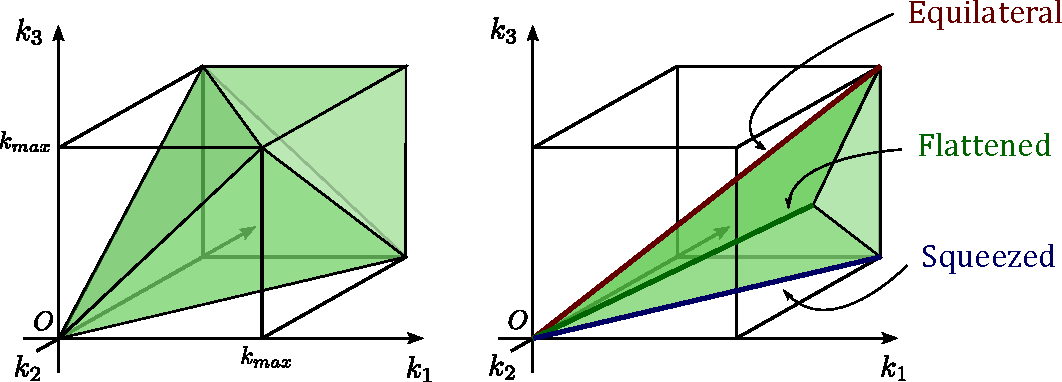
\includegraphics[width=1.0\textwidth]{tetrapyd.pdf}
	\caption{Tetrapyd domain in which the shape functions are defined. Left: the full region specified by triangle inequalities and an upper bound $k_{max}$. Right: one sixth slice of the tetrapyd from which shape functions are uniquely determined by symmetry in the $k$'s. Edges representing the equilateral, flattened and squeezed configurations are annotated.}
	\label{fig:tetrapyd}
\end{figure}

We follow \cite{Fergusson2010general} and denote this domain consisting of two tetrahedrons glued together as `tetrapyd'. Note that all shape functions of interest are symmetric in the $k$'s, so we may restrict our interest to a region where $k_1 \ge k_2 \ge k_3$ (right of Figure \ref{fig:tetrapyd}). We dub the resulting tetrahedron with one sixth the original volume `the sliced' tetrapyd, somewhat unoriginally. The three main types of triangle configurations correspond to three edges of the sliced tetrapyd: equilateral ($k_1=k_2=k_3$), flattened ($k_1 = k_2 + k_3$), and squeezed ($k_1 = k_2 \gg k_3$). \footnote{To be precise, the edges for flattened represent $k_1/2 = k_2 = k_3$, and the squeezed one is defined as $k_1=k_2$, $k_3=0$. The edges by themselves are unphysical, but points near these lines correspond to the limits described.} Figure \ref{fig:Legendre_basis_functions_3D} shows some of the Legendre basis functions plotted in three dimensions.

\begin{figure}
	\centering    
	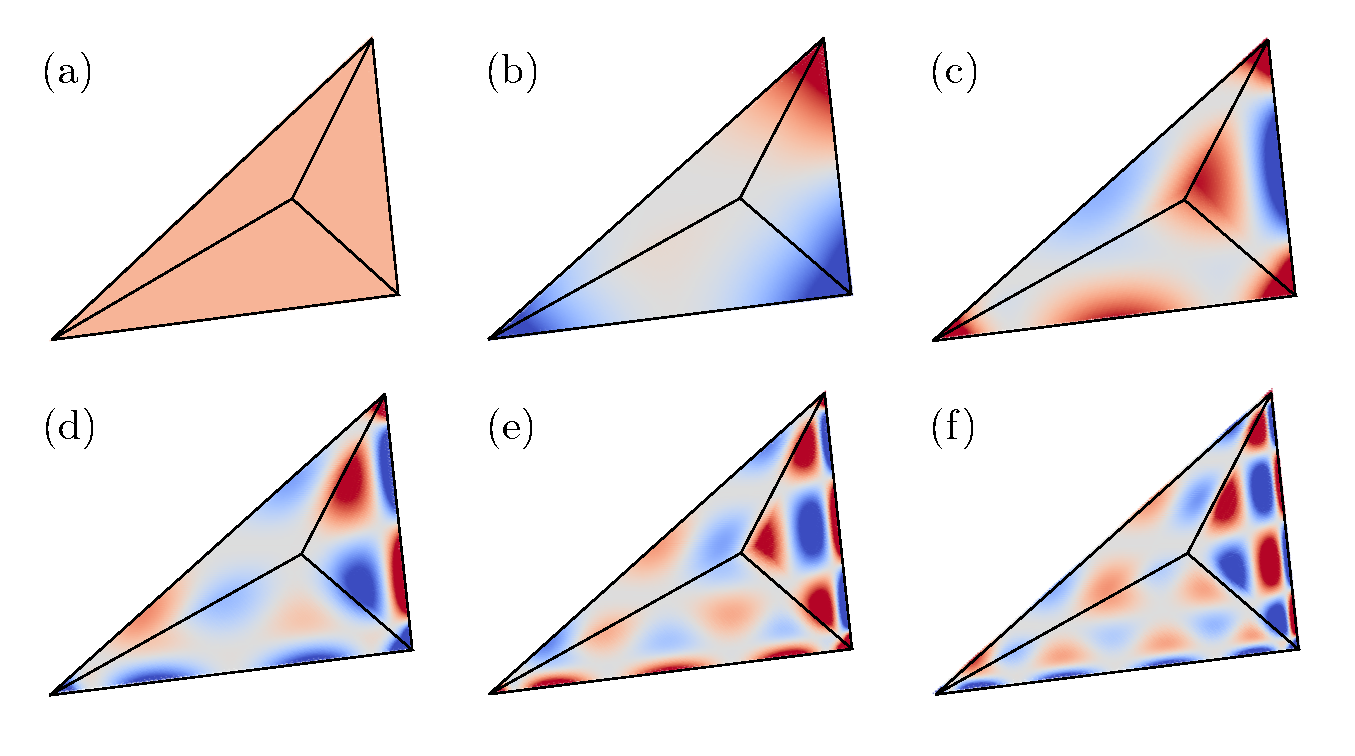
\includegraphics[width=1.0\textwidth]{legendre_modes_3D_final.pdf}
	\caption{Examples of our Legendre basis functions, evaluated on the sliced tetrapyd domain shown in Figure \ref{fig:tetrapyd}. Functions are defined as $Q_{p_1 p_2 p_3}(k_1,k_2,k_3) := P_{p_1}(k_1) P_{p_2}(k_2) P_{p_3}(k_3)$, where $P_l(k)$ are Legendre polynomials. Here we plot $p_1 = p_2 = p_3 = p$, where $p$ equals (a) $0$, (b) $1$, (c) $2$, (d) $3$, (e) $4$, and (f) $5$. A single colour map is used across plots: red and blue correspond to $+1$ and $-1$, respectively.}	
	\label{fig:Legendre_basis_functions_3D}
\end{figure}

Let $V_{\vv{k}}$ be the subset of $\mathbb{R}^3$ representing the sliced tetrapyd. By choosing a natural inner product
\begin{align}
	\left< S_1, S_2 \right> = \int_{V_{\vv{k}}} d^3\vv{k} \;\; S_1(\vv{k}) S_2(\vv{k}), \label{eqn:tetrapyd_inner_product}
\end{align}
we restrict our attention to an $L^2$ space defined on $V_{\vv{k}}$: a vector space consisting of square-integrable functions.
\footnote{Note that the local shape function $S(k_1,k_2,k_3) = (k_1^2 / k_2 k_3 + \text{2 cyc.})$ is not in fact square-integrable due to its divergence as $k_i \rightarrow 0$. We work around this problem by prescribing a lower bound $k \ge k_{min}$, which is also the case in numerical calculations.}
A set of three-dimensional basis functions $Q_{\vv{p}}$ with size $N$ spans a subspace $U_{Q} \subset L^2(V_{\vv{k}})$ of dimension at most $N$.

Using this notation, expanding a given shape function $S$ with respect to a basis set $Q$ is equivalent to finding its orthogonal projection into $U_{Q}$;
\begin{align}
	&S = S^{\parallel} + S^{\perp}, \;\;\;\text{where} \\
	&S^{\parallel} \in U_Q \;\;\;\;\text{and} \;\;\; \left< S^{\perp}, Q' \right> = 0, \; \forall Q' \in U_Q.
\end{align}
As long as $\left\| S^\perp \right\| \ll \left\| S \right\|$, we may approximate
\begin{align}
	S \approx S^\parallel = \sum_{\vv{p}} \alpha_{\vv{p}} Q_{\vv{p}}.  \label{eqn:primordial_basis_projection}
\end{align}
The decomposition coefficients $\alpha$ are obtained by taking inner product with $Q_{\vv{p}}$ on both sides.
\begin{align}
	\left< S, Q_\vv{p} \right> = \left< Q_\vv{p}, Q_{\vv{p}'} \right> \alpha_{\vv{p}'}. \label{eqn:primordial_basis_expansion_SQ_and_QQ}
\end{align}
From above, we can compute $\alpha_\vv{p}$ by inverting the matrix $\Gamma_{\vv{p} \vv{p}'} = \left< Q_\vv{p}, Q_{\vv{p}'} \right>$. Alternatively, orthonormalising the basis with respect to the inner product $\left< , \right>$ turns $\Gamma$ to an identity matrix, trivialising the inversion process.

We rewrote the formalism using linear analysis language here to emphasize two aspects of our primordial basis expansion. First, even though we choose a simple inner product (\ref{eqn:tetrapyd_inner_product}) for now, the method is completely general, and we may freely choose a different inner product. For example, non-unit weights $w(\vv{k})$ can be included in the integrand, and/or the domain of integration may be changed. Doing so alters how we decompose shape functions in terms of our basis.

Second, we highlight the fact that basis expansion is in essence a minimisation problem with respect to chosen inner product, which is often oblivious of late-time physics. Orthogonal projection of $S$ to subspace $U_Q$ is a point in $U_Q$ which has minimal distance to $S$: $\left\| S - S^\parallel \right\|$ is minimised. Obtained $S^\parallel$, however, is not necessarily the best description of $S$ when we consider their late-time counterparts in $l$ space. Some errors with small norm $\left\| \Delta S \right\|$ might get enhanced when convolved with transfer functions, yielding large reduced bispectrum $\Delta b_{l_1 l_2 l_3}$. Meanwhile, sometimes large differences in $S$ are completely unobservable late-time and provide mostly identical constraints on $f_{NL}$.

With these points in mind, we define metrics to compare shape functions in primordial space;
\begin{align}
	\text{Corr}(S_1, S_2) &:= \frac{\left< S_1, S_2 \right>}{ \sqrt{ \left< S_1, S_1 \right> \left< S_2, S_2 \right> } }, \\
	\epsilon^2(S_1, S_2) &:= \frac{\left< S_1 - S_2, S_1 - S_2 \right> }{\sqrt{\left< S_1, S_1 \right> \left< S_2, S_2 \right>}}.
\end{align}
Corr$(S_1,S_2)$ measures correlation between the two shapes and is independent of the normalisation. $\epsilon(S_1,S_2)$ is the distance between two shapes, which reduces to $\sqrt{2 - 2\;\text{Corr}(S_1,S_2)}$ when $S_1$ and $S_2$ have equal amplitude. We use both of these values to test if our primordial basis expansion has converged to target shape function. 

Inverting the matrix $\Gamma_{\vv{p} \vv{p}'} = \left< Q_\vv{p}, Q_{\vv{p}'} \right>$ in \eqref{eqn:primordial_basis_expansion_SQ_and_QQ} can be tricky in practice. The $p_{max}^3 \times p_{max}^3$ matrix is not only large in size for high $p_{max}$, but also near singular. Some of the three-dimensional mode functions $Q_\vv{p}$ become linearly dependent within tetrapyd even if they are constructed from independent modes in one dimension. Presence of such degenerate modes induces severe numerical instability during inversion.

For our Legendre basis, we use a small trick to get around this problem. Motivated by the fact that Legendre polynomials form an orthogonal basis in one dimension, we extend the domain of integral in the inner product \eqref{eqn:tetrapyd_inner_product} to a cube containing the tetrapyd instead. Most template shape functions have an analytic form and can easily be extended in this region. As long as $\int dk \; q_p(k) q_{p'}(k) = \delta_{pp'}$, the decomposed coefficients for given $S$ can be found by
\begin{align}
	\alpha^{(t)}_{p_1 p_2 p_3} = \int dk_1 \int dk_2 \int dk_3 \; S^{(t)}(k_1, k_2, k_3) q_{p_1}(k_1) q_{p_2}(k_2) q_{p_3}(k_3). \label{eqn:basis_expansion}
\end{align}
Note that the three-dimensional integral can now be split into three separate one-dimensional integrals in range $[k_{min}, k_{max}]$. By performing the three integrals one by one, we obtain a numerically stable algorithm that is fast and memory efficient. Decomposing a shape evaluated on $1000^3$ $k$ grid points with respect to $30^3$ Legendre basis functions only takes a few seconds in our \textsc{C} code.

After we obtain coefficients from (\ref{eqn:basis_expansion}), we evaluate accuracy of the expansion using the inner product defined in tetrapyd because it is the only physical region where our shape function matters. Since the cube includes tetrapyd, good convergence in cube guarantees small error within the tetrapyd in most cases. The only exception is when the target shape function blows up outside tetrapyd. We will see such examples in later sections.


\section{Implementation and optimisation} \label{section:implementation}

CMB bispectrum estimation is a numerically challenging task. All existing approaches exploit the separability of multi-dimensional integrals to reduce computational complexity, because it is practically impossible otherwise. Planck analysis provided constraints to primordial non-Gaussianity from various bispectrum templates, but having limited computing resources was what stopped us from exploring further. Numerous shapes such as complex oscillatory models have been outside our reach despite their being theoretically well-motivated.

The CMB-BEst formalism significantly reduces the amount of computation needed for the CMB bispectrum estimation. Obtaining the linear term $\beta^{lin}$ in (\ref{def:beta_linear}), however, is still prohibitively expensive unless thoroughly optimised. Performance is especially crucial here since it directly affects the breadth of models we can cover; the faster the code, the higher number of modes we can have, and the more shapes we can expand in our basis accurately.

In this section, we provide details for various aspects of our optimisation process: algorithm design, parallel computing, and data locality improvements. Final specifications and data files used are outlined at the end.

Throughout this section we will treat the functions of interest as discrete arrays. Our notations for indices and their limits are summarised in Table \ref{table:index_conventions}. We adopt simple trapezoidal rule for most numerical integrals. For the $\mu$ integral in (\ref{def:gamma}), however, we use Gauss-Legendre quadrature computed from the public code \textsc{Quadpts} \cite{Hale2013} due to highly oscillatory and unstable nature of the integral. Multi-dimensional arrays are stored in the row major order following the \textsc{C} convention for efficiency. We use the \textsc{Healpix} library \cite{Gorski2005healpix} for pixelisation of the sky, which includes \textsc{libsharp} \cite{Reinecke2013libsharp} library for Spherical Harmonic Transforms (SHTs).

\begin{table}[htbp]
	\caption{Our index conventions for discretised arrays and their sizes.}
	\centering
	\label{table:index_conventions}
	\renewcommand{\arraystretch}{1.5} 
	\begin{tabular}{m{0.1\textwidth}  m{0.1\textwidth}  m{0.7\textwidth}} \toprule
		Index & Range & Description \\
		
		\midrule
		$r$ & $[0, N_r)$ & Line-of-sight integral $r$ grid index. \\
		
		$p, p_j$ & $[0, p_{max})$ & Mode number. $p_j$ is a shorthand for $(p_1, p_2, p_3)$. \\
		
		$i,j$ & $[0, N_{sims}]$ & Map number. Index $i=0$ corresponds to the observed CMB map, while $i>0$ are for simulated Gaussian maps. \\			
		
		$n$ & $[0, N_{pix})$ & Map pixel number. \\ 
		
		$l,m$ & $[0, l_{max})$ & Spherical harmonic multipole moments. Note $-l \le m \le l$. \\
		
		$\mu$ & $[0, N_\mu)$ & Gauss-Legendre quadrature $\mu$ grid index. \\
		
		\bottomrule
	\end{tabular}
\end{table}

\subsection{Algorithm}

Our goal is to compute three key quantities: $\Gamma$ (\ref{def:gamma}), $\beta^{cub}$ (\ref{def:beta_cubic}), and $\beta^{lin}$ (\ref{def:beta_linear}). The matrix $\Gamma$ allows us to find the normalisation factor $N$ for a given theoretical template, while the two $\beta$'s provide the amplitude of $f_{NL}$ for each CMB maps and simulations used, up to normalisation.

In most cases of interest, the bottleneck point of our pipeline is computing the linear term $\beta^{lin}$. Even though the $\Gamma$ matrix computation through (\ref{def:gamma}) grows more rapidly with the number of basis functions ($\propto p_{max}^6$) than the $\beta$'s ($\propto p_{max}^3$), it does not involve operations with high-definition maps and remains subdominant in terms of total cost.

We dedicate this section to explain our algorithm design for $\beta$ computation in detail. The discretised versions of (\ref{def:beta_cubic}-\ref{def:beta_linear}) are given by
\begin{align}
	\beta^{cub}(i, p_1,p_2,p_3) &= \sum_r \sum_n \; M(r, i, p_1, n) \cdot M(r, i, p_2, n) \cdot M(r, i, p_3, n), \\
	\beta^{lin}(i, p_1,p_2,p_3) &= \sum_r \sum_{j \neq i} \sum_n \; M(r, j, p_1, n) \cdot M(r, j, p_2, n) \cdot M(r, i, p_3, n).
\end{align}
The order of indices are chosen such that later calculations have optimal memory layouts. Some integral weights and factors are absorbed into arrays for brevity.

Note that the data arrays for different values of $r$ are completely independent to each other. This provides us a natural way to distribute tasks. We compute and save contributions to $\beta$'s for each $r$ separately. The summation over $r$ is performed in the end. Therefore, throughout the rest of this chapter, we assume that $r$ is fixed and drop the $r$ dependence in descriptions of our algorithms.

The filtered map arrays $M(i,p,n)$ are obtained as follows. A given map $i$ is first transformed in to spherical harmonic coefficients $a^{(i)}(l,m)$s via SHT. We then compute $\tilde{q}_(p,l) * a(i,l,m) / C(l)$ from (\ref{def:filtered_maps}), which is fed into reverse SHT to synthesise the filtered maps.

As a rough guide to the size of each summations, we typically have $N_{sim} \approx 150$ simulations, $p_{max} = 30$ modes, and $N_{pix} = 50,331,648$ pixels. \footnote{This value corresponds to $N_{side} = 2048$ in Healpix. $N_{pix} = 12 N_{side}^2$} Considering the fact that one double-precision array of size $\sim 50$ million pixels takes about 400MB of memory space, this is indeed a task for supercomputers.

Our first and the most straightforward method of computing $\beta$s are outlined in Algorithm \ref{alg:beta_first_attempt}. Computational complexity of each innermost loop is denoted on the right hand side.

\begin{algorithm}[htbp]
	\caption{Computing $\beta$s: the na\"ive method}
	\label{alg:beta_first_attempt}
	\begin{algorithmic}[1] % The number tells where the line numbering should start	
		\State Allocate $M(i,p,n)$
		\Comment{Memory $\sim N_{sims} \cdot p_{max} \cdot N_{pix}$}

		\\
		\For{each map $i$}
			\For{each mode $p$}
			\Comment{$O(N_{sims} \cdot p_{max} \cdot N_{pix}^{3/2})$}
				\State \textbf{compute} $M(i,p,n)$ by SHT
			\EndFor
		\EndFor \Comment{$M(i,p,n)$ ready}
		\\
		
		\For{each map $i$}
			\For{each set of modes $(p_1,p_2,p_3)$}
				\For{each pixel $n$}
				\Comment{$O(N_{sims} \cdot p_{max}^3 \cdot N_{pix})$}
					\State $\beta^{cub}(i, p_1, p_2, p_3) \pluseq M(i,p_1,n) \cdot M(i,p_2,n) \cdot M(i,p_3,n)$
				\EndFor
			\EndFor
		\EndFor

		\\	
		\For{each map $i$}
			\For{each map $j \neq i$}
				\For{each set of modes $(p_1,p_2,p_3)$}
					\For{each pixel $n$}
					\Comment{$O(N_{sims}^2 \cdot p_{max}^3 \cdot N_{pix})$}
						\State $\beta^{lin}(i, p_1, p_2, p_3) \pluseq M(j,p_1,n) \cdot M(j,p_2,n) \cdot M(i,p_3,n)$
					\EndFor
				\EndFor
			\EndFor
		\EndFor

	\end{algorithmic}
\end{algorithm}

Here, we first obtain the filtered maps $M(i,p,n)$ via SHT for each map and modes. The full results are stored in memory. Next, we iterate through each map and set of modes $(p_1, p_2, p_3)$ and sum over each of the map pixels to obtain $\beta^{cub}$ and $\beta^{lin}$. Symmetries in the indices are respected; we only loop over $(p_1,p_2,p_3)$ satisfying $p_1\ge p_2$ for the linear terms, and $p_1\ge p_2\ge p_3$ for the cubic ones.

SHT typically scales as $\propto l_{max}^3$, where $l_{max}$ is the maximum degree of spherical harmonic functions used. The total number of pixels $N_{pix}$ grows $\propto l_{max}^2$ when chosen appropriately for resolution, hence the SHT costs $O(N_{sims}\cdot p_{max} \cdot N_{pix}^{3/2})$. The most expensive part of this algorithm is still the loop where we calculate the linear term, which scales as $O(N_{sims}^2 \cdot p_{max}^3 \cdot N_{pix})$.

Our first major optimisation comes from the observation that we may swap the order of summations to reduce the computation. By precomputing $C(p_1, p_2, n) = \sum_j M(j,p_1,n) \cdot M(j,p_2,n)$, we require one fewer loop over maps for $\beta^{lin}$, leading to a factor of $N_{sims}\sim150$ improvement. Algorithm \ref{alg:beta_second_attempt} shows a pseudocode for this method.

\begin{algorithm}[htbp]
	\caption{Computing $\beta$s: optimised for computation}
	\label{alg:beta_second_attempt}
	\begin{algorithmic}[1] % The number tells where the line numbering should start	
		\State Allocate $M(i,p,n)$ \Comment{Memory $\sim N_{sims} \cdot p_{max} \cdot N_{pix}$}
		\State Allocate $C(p_1,p_2,n)$ \Comment{Memory $\sim p_{max}^2 \cdot N_{pix}$}
		\\
		\For{each map $i$}
			\For{each mode $p$}
				\Comment{$O(N_{sims} \cdot p_{max} \cdot N_{pix}^{3/2})$}
				\State \textbf{compute} $M(i,p,n)$ by SHT
			\EndFor
		\EndFor \Comment{$M(i,p,n)$ ready}
		\\
		\For{each map $j$}
			\For{each pair of modes $(p_1,p_2)$}
				\For{each pixel $n$}
					\Comment{$O(N_{sims} \cdot p_{max}^2 \cdot N_{pix})$}
					\State $C(p_1,p_2,n) \pluseq M(j,p_1,n) \cdot M(j,p_2,n)$
				\EndFor
			\EndFor
		\EndFor \Comment{$C(p_1,p_2,n)$ ready}
		\\
		\For{each map $i$}
			\For{each set of modes $(p_1,p_2,p_3)$}
				\For{each pixel $n$}
					\Comment{$O(N_{sims} \cdot p_{max}^3 \cdot N_{pix})$}
					\State $\beta^{cub}(i, p_1, p_2, p_3) \pluseq M(i, p_1, n) \cdot M(i, p_2, n) \cdot M(i, p_3, n)$
					\State $\beta^{lin}(i, p_1, p_2, p_3) \pluseq C(p_1, p_2, n) \cdot M(i, p_3, n)$
				\EndFor
			\EndFor
		\EndFor
	\end{algorithmic}
\end{algorithm}

Note that the resulting sum fo $\beta^{lin}$ includes an unwanted contribution from the case where $j=i$, since $C(p_1,p_2,n)$ is obtained by summing over all maps. Thankfully, this extra contribution is exactly equal to the cubic term. We just have to subtract $\beta^{cub}$ from the total sum to get the correct value of $\beta^{lin}$.

We shaved off a whole loop at the cost of extra memory usage. For our purposes $N_{sims} \sim 150 > p_{max} = 30$, so the additional space required for $C(p_1,p_2,n)$ is relatively small compared to $M(i,p,n)$. The symmetry in $p_1$ and $p_2$ also means that we only need to store $p_{max}(p_{max}+1)/2$ maps instead of $p_{max}^2$ for $C$.

Our next challenge is the amount of memory required to save $M(i,p,n)$. For the parameters mentioned above, this is $\approx 1.8$TB, which is quite significant. Though it is not impossible to find supercomputing systems which can accommodate such large arrays, reduction in memory usage would be highly beneficial. We seek to achieve it while keeping the overall computational complexity to be $O(N_{sims} \cdot p_{max}^3 \cdot N_{pix})$ as before.

We observe that most summations are done for a single map $i$. The array $C(p_1,p_2,n)$ is required to be computed before the main loop for $\beta^{lin}$, but otherwise there are no `mixing' between the maps. We exploited this fact to develop Algorithm \ref{alg:beta_third_attempt}.

\begin{algorithm}[htbp]
	\caption{Computing $\beta$s: fast and memory efficient}
	\label{alg:beta_third_attempt}
	\begin{algorithmic}[1] % The number tells where the line numbering should start	
		\State Allocate $m(p,n)$ \Comment{Memory $\sim p_{max} \cdot N_{pix}$}
		\State Allocate $C(p_1,p_2,n)$ \Comment{Memory $\sim p_{max} \cdot p_{max} \cdot N_{pix}$}
		\\
		\For{each map $i$}
			\For{each mode $p$}
				\Comment{$O(N_{sims} \cdot p_{max} \cdot N_{pix}^{3/2})$}
				\State \textbf{compute} $M(i,p,n)$ by SHT and store in $m(p,n)$
			\EndFor
			\\
			\For{each pair of modes $(p_1,p_2)$}
				\For{each pixel $n$}
				\Comment{$O(N_{sims} \cdot p_{max}^2 \cdot N_{pix})$}
					\State $C(p_1,p_2,n) \pluseq m(p_1,n) \cdot m(p_2,n)$
				\EndFor
			\EndFor
		\EndFor
		\Comment{$C(p_1,p_2,n)$ ready}
		\\
		\For{each map $i$}
			\For{each of mode $p$}
				\Comment{$O(N_{sims} \cdot p_{max} \cdot N_{pix}^{3/2})$}
				\State \textbf{compute} $M(i,p,n)$ by SHT and store in $m(p,n)$
			\EndFor
			\\
			\For{each set of modes $(p_1,p_2,p_3)$}		\label{alg:thrid_attempt_main_loop}	
				\For{each pixel $n$}
					\Comment{$O(N_{sims} \cdot p_{max}^3 \cdot N_{pix})$}	
					\State $\beta^{cub}(i, p_1, p_2, p_3) \pluseq m(p_1,n) \cdot m(p_2,n) \cdot m(p_3,n)$
					\State $\beta^{lin}(i, p_1, p_2, p_3) \pluseq C(p_1, p_2, n) \cdot m( p_3, n)$
				\EndFor
			\EndFor
		\EndFor
	\end{algorithmic}
\end{algorithm}

Algorithm \ref{alg:beta_third_attempt} dramatically reduces the amount of memory required, at the cost of doubling the SHTs for computing $M(i,p,n)$s. The first time through, SHT results from each map are used to find $C(p_1,p_2,n)$. After a full loop over maps we have $C(p_1,p_2,n)$ ready, another set of SHTs for each map allows us to obtain the $\beta$'s.

SHTs have subdominant contribution to the total computation time even after becoming doubled in number. One of the main strengths of Algorithm \ref{alg:beta_third_attempt} is that both the memory and computation time scale linearly with the number of simulations used, $N_{sims}$. In the future when a larger number of Gaussian simulations are required to acquire a more accurate estimate of the linear term, it is straightforward to adapt our method accordingly.

We choose Algorithm \ref{alg:beta_third_attempt} to be our main method of computing $\beta$'s for CMB-BEst.

\subsection{Parallel computing}

% Do I need more computing related references here maybe?

In order to fully benefit from the modern computer architecture, parallel computing is a must. In this section, we outline how CMB-BEst was parallelised for optimal performance on supercomputers.

Following \cite{Jeffers2016intel}, we discuss parallelism in three different levels: domain, thread, and data. They mostly correspond to nodes, cores, and registers in modern computer clusters. Each level has distinct characteristics which make them ideal for different parallelisation techniques. We make the full use of each level in our methodology.

\textit{Domain} parallelism refers to dividing the task into many domains where each domain entails heavy computation, while having limited data communication between them. Since the domains are largely independent, Message Passing Interface (MPI) is a suitable tool for parallelisation. MPI is a communication protocol where many instances (`ranks') of the same code may transfer data while running separately from each other. A perfect example of domain parallelism in CMB-BEst would be our line-of-sight integration over $r$. Almost no data are shared between different $r$s, despite the heavy computational cost from map operations within each domain. CMB-BEst therefore scales well with the number of MPI ranks.

\textit{Thread} parallelism opportunities arise when there are many independent computational tasks on a single set of data. Most modern supercomputers use multi-core processors. Each core, or processing units, can run one or more threads, executing instructions independently from each other while sharing memory space. Note that MPI would not be as effective here due to the large amount of data sharing needed; ranks have to either continuously communicate with each other, or store individual copies of the data. This type of parallelism is extremely common in many applications, including SHTs and map integrations in CMB-BEst. Open Multi-Processing (OpenMP) is one of the most popular implementations of multi-threading publicly available. We utilise the \textsc{C} OpenMP interface in our code. 

\textit{Data} parallelism applies when same arithmetic operations are applied to multiple data items, ideally adjacent in memory space. This type of parallel processing is called SIMD: Single Instruction, Multiple Data. Many procedures involving large arrays fall into this category. We use Advanced Vector Extensions (AVX) supported by Intel processors to exploit data parallelism in CMB-BEst, especially for operations involving large (filtered) map arrays. In particular, Intel's Xeon Phi series implement AVX-512, where 512-bit registers hold up to 8 double-precision floating numbers. A single instruction can be applied on all of them at once in a single clock cycle, providing a major boost to computation speed. We explicitly align large arrays in memory for optimal vectorisation performance.

Table \ref{table:three_levels_of_parallelism} summarises discussions in this section.

\begin{table}[h]
	\caption{Three levels of parallelism utilised in CMB-BEst. The levels and characteristics are chosen based on \cite{Jeffers2016intel}.}
	\centering
	\label{table:three_levels_of_parallelism}
	\renewcommand{\arraystretch}{1.5} 
	\begin{tabular}{m{0.12\textwidth}   m{0.35\textwidth}   m{0.15\textwidth}   m{0.3\textwidth}} \toprule
		 & Characteristics & Methods & Utilisation \\
		
		\midrule
		Domain \newline Parallelism &
		\begin{itemize}[leftmargin=*]
			\item Limited data communication between domains
			\item Heavy computation within the domain
		\end{itemize} &
		MPI &
		\begin{itemize}[leftmargin=*]
			\item Line of sight $r$ integration split into independent tasks
		\end{itemize}  \\
	
		\midrule
		Thread \newline Parallelism &
		\begin{itemize}[leftmargin=*]
			\item Data sharing between threads
			\item High proportion of independent tasks
		\end{itemize} &
		OpenMP &
		\begin{itemize}[leftmargin=*]
			\item SHT
			\item Map patches divided across threads
		\end{itemize}  \\	
	
		\midrule
		Data \newline Parallelism &
		\begin{itemize}[leftmargin=*]
			\item Same operation applied to multiple data items
		\end{itemize} &
		SIMD &
		\begin{itemize}[leftmargin=*]
			\item Map pixel integration vectorised using AVX-512
			\item Data vectors explicitly aligned in memory for optimal performance 
		\end{itemize} \\	
			
		\bottomrule
	\end{tabular}
\end{table}

\subsection{Data locality}

We implemented Algorithm \ref{alg:beta_third_attempt} and profiled using the Intel VTune Amplifier. Our program was found to be memory-bound, which means that its speed is limited mainly by the amount of memory available and the speed of memory access. The CPU speed, rate of the file I/O, and MPI communication all have subdominant contributions in comparison. This is somewhat expected, since our method deals with large map arrays. The number of operations on each data element is small compared to the size of data, causing the CPUs to be `starved' for data to work on most of the time. Our final set of optimisation focusses on improving memory access patterns.

CPUs of most modern computers contain a small amount of memory attached to them called \textit{cache}. Recently used data and instructions are stored in cache memory so that reusing them is more efficient; accessing cache is much faster than loading from the main, larger memory often shared with other CPUs. Cache is often divided into multiple levels. The smallest and fastest is L1 cache, which is the first level a CPU checks for data. When the required data is not stored in L1 cache, a \textit{cache miss} occurs. The system then has to look further down the cache levels to fetch the wanted data, incurring a large time loss. It is therefore crucial to reuse data as many times as possible before it is lost from cache.

Furthermore, the cache `caches' memory locations in units of cache lines, or chunks of memory containing multiple data elements. Accessing memory locally therefore significantly increases the chance of cache hits, boosting overall performance. Array operations, for example, are optimised when they are stored in consecutive memory locations due to this fact.

CMB-BEst has been modified in two ways to improve data locality and memory performance. The first one was simple yet effective; we made sure to initialise large arrays within the same OpenMP construct as the main computation loop. This guarantees the physical memory of array elements to be allocated near the cores where they are going to be used in. Memory access during the main computation loop is therefore much faster than otherwise. Systems with non-uniform memory access (NUMA) especially benefits from this method. For CMB-BEst, we gained 2 times speed-up compared to when a single master thread initialised the entire array.

The second optimisation centres around \textit{cache blocking}, a technique used to maximise data reuse. Let us focus on the main computation loop in Algorithm \ref{alg:beta_third_attempt}:

\begin{algorithmic}
	\For{each set of modes $(p_1,p_2,p_3)$}
		\For{each pixel $n$}
			\State $\beta^{cub}(i, p_1, p_2, p_3) \pluseq m(p_1,n) \cdot m(p_2,n) \cdot m(p_3,n)$
			\State $\beta^{lin}(i, p_1, p_2, p_3) \pluseq C(p_1, p_2, n) \cdot m( p_3, n)$
		\EndFor
	\EndFor
\end{algorithmic}

In every loop over the set of modes $(p_1, p_2, p_3)$, four large arrays are read from memory: $m(p_1,\cdot)$, $m(p_2,\cdot)$, $m(p_3,\cdot)$, and $C(p_1, p_2, \cdot)$. Each of them take up around 400MB of memory. Since their size is greater than the cache storage capacity, data in the front of them are gone from cache by the time a loop over $n$ completes. All four arrays will then have to be loaded from main memory again when the next iteration starts.

Suppose that the map arrays had smaller size and all of them fit in one of the cache levels instead. After one loop iteration over $n$ for $(p_1, p_2, p_3)$, the arrays now remain in cache. Then the next loop on $(p_1, p_2, p_3+1)$ begins, and the arrays $m(p_1,\cdot)$, $m(p_2,\cdot)$, and $C(p_1,p_2,\cdot)$ are required again for computation. They can now be accessed from cache, which saves significant amount of time. We see that each data element is reused multiple times before discarded from cache in this case.

Motivated by these facts, we divide the map array into equally sized blocks so that each patch can now fit inside the cache memory. We restructure the loop as follows.

\begin{algorithmic}
	\For{each block $b$}
		\For{each set of modes $(p_1,p_2,p_3)$}
			\For{each pixel $n'$ in block}
				\State $\beta^{cub}(i, p_1, p_2, p_3) \pluseq m(p_1,n') \cdot m(p_2,n') \cdot m(p_3,n')$
				\State $\beta^{lin}(i, p_1, p_2, p_3) \pluseq C(p_1, p_2, n') \cdot m( p_3, n')$
			\EndFor
		\EndFor
	\EndFor
\end{algorithmic}

The new pixel numbers are calculated as $n' = B \cdot b + n$, where $B$ is the size of each block and $0 \le n < B$. We have not changed the total number of arithmetic operations required, so the computational complexity remains constant. Meanwhile, data locality within each block is greatly improved, as each of the blocked arrays are now small enough to fit in cache. Each data element is accessed in closer succession temporarily as well.

One caveat here is that having too many blocks may degrade performance. There exist non-negligible overhead coming from an extra \textit{for} loop and the OpenMP construct used over $n'$. The block size divided by number of cores should not be smaller than the size of cache lines either. The optimal size of cache blocks depends on the memory architecture of the processor used. This often needs to be found empirically.

Figure (\ref{fig:cache_block_optimisation}) shows how runtime of a small test code varies with the number of cache blocks used. The code was run on the Intel Gold 6154 processor, which is an 18-core high performance chip with total L1, L2, and L3 cache memory sizes of 1.125MiB, 18MiB, and 24.74MiB, respectively \cite{intel_data_sheet}. Even though some parameters such $N_{sims}$ are tuned down for faster testing, this is representative of the full computation.

\begin{figure}[htbp!] 
	\centering    
	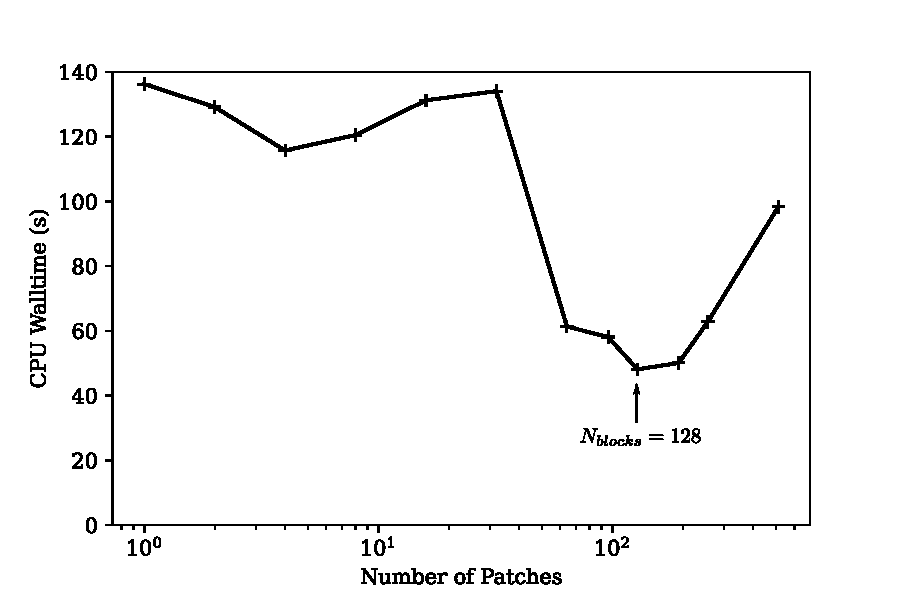
\includegraphics[width=0.8\textwidth]{cache_block_optimisation_annotated.pdf}
	\caption[Cache block optimisation]{Cache block optimisation. Total wall time of a test code for computing $\beta$s was measured while varying the number of cache blocks used. Having 128 blocks is optimal for the 18-core Intel Gold 6154 processor.}
	\label{fig:cache_block_optimisation}
\end{figure}

We find a significant improvement in performance moving from 32 to 48 blocks when the block size drops from 12MiB to 8MiB. This is precisely when three blocks are allowed fit in L3 cache (24.7MiB) at the same time. Improved data locality dramatically reduces time spent on memory access as we expected. The optimal number of blocks was found to be 128; each segment contains about 400,000 elements and takes up 3MiB of memory, which is 1/6 and 1/8 of L2 and L3 cache size, respectively. We gain roughly three times speed-up compared to the original code without cache blocking.

Algorithm \ref{alg:beta_final_algorithm} summarises our final implementation of $\beta$ computation code, now with cache blocking and OpenMP construct indicators.

\begin{algorithm}[htbp]
	\caption{Computing $\beta$s: our final implementation}
	\label{alg:beta_final_algorithm}
	\begin{algorithmic}[1] % The number tells where the line numbering should start	
		\State Allocate $m(p,n)$ 
		\State Allocate $C(p_1,p_2,n)$ 
		\\\Comment{Both initialised within OpenMP construct over $n$}

		\For{each map $i$}
		\For{each mode $p$}
		\State \textbf{compute} $M(i,p,n)$ by SHT and store in $m(p,n)$
		\Comment{OpenMP within SHT}
		\EndFor
		\\
		\For{each block $b$}
		\For{each pair of modes $(p_1,p_2)$}
		\For{each pixel $n'$ in block}
		\Comment{OpenMP \textit{for} construct}
		\State $C(p_1,p_2,n') \pluseq m(p_1,n') \cdot m(p_2,n')$
		\EndFor
		\EndFor
		\EndFor
		\EndFor
		\Comment{$C(p_1,p_2,n)$ ready}
		\\
		\For{each map $i$}
		\For{each of mode $p$}
		\State \textbf{compute} $M(i,p,n)$ by SHT and store in $m(p,n)$
		\Comment{OpenMP within SHT}
		\EndFor
		\\
		\For{each block $b$}
		\For{each set of modes $(p_1,p_2,p_3)$}		
		\For{each pixel $n'$ in block}
		\Comment{OpenMP \textit{for} construct}
		\State $\beta^{cub}(i, p_1, p_2, p_3) \pluseq m(p_1,n') \cdot m(p_2,n') \cdot m(p_3,n')$
		\State $\beta^{lin}(i, p_1, p_2, p_3) \pluseq C(p_1, p_2, n') \cdot m( p_3, n')$
		\EndFor
		\EndFor
		\EndFor
		\EndFor
	\end{algorithmic}
\end{algorithm}

\section{Validation} \label{section:validation}

CMB bispectrum estimation is not only computationally challenging but also prone to numerical instabilities unless implemented carefully. We invested considerable amount of time after the development of CMB-BEst in validating various aspects of the code. We highlight some of our validation efforts in this section, checking consistency within the program itself (section \ref{section:internal_consistency}) and against existing codes such as Modal \cite{Fergusson2012} (section \ref{section:consistency_with_Planck}).

\subsection{Internal consistency checks} \label{section:internal_consistency}

CMB-BEst is a general code where one can freely choose a set of basis functions. Three of our main options are the `KSW' basis (\ref{eqn:KSW_basis}), `Legendre' basis (\ref{eqn:Legendre_basis_no_inv_k}, augmented with $q(k)=k^{n_s-2}$) as discussed previously in Section \ref{section:basis_functions}, and Fourier basis (\ref{eqn:Fourier_basis}). Both KSW and Legendre basis sets can cover the standard templates: local, equilateral, and orthogonal (see e.g., \cite{PlanckCollaboration2013} for definitions). The KSW basis provides an exact form to the three templates by choosing appropriate powers of $k$ as its basis elements. On the other hand, the templates are expanded in terms of separable Legendre polynomials up to some fixed degree $p_{max}$ for the Legendre basis. As long as $p_{max}$ is sufficiently large, most smooth bispectrum shapes can be represented accurately. 

Our first consistency check is shown in Figure \ref{fig:map_by_map_Legendre_KSW}, where we compare the $f_{NL}$ estimates from the Planck 2018 CMB map and 140 full focal plane (FFP10) realistic Gaussian simulations \cite{PlanckCollaboration2015simulations}. We use CMB maps obtained through the SMICA component separation method \cite{Cardoso2008component, PlanckCollaboration2013ComponentSeparation}. On the left hand side are scatter plots of $f_{NL}$ values obtained using each of the two basis sets. In an ideal case where the two estimates are identical for every test maps, all the points would lie on a straight line given by $y=x$. Drawn in dashed red line is the best linear fit to the data. Its slope, intercept, and the $R$-squared value are annotated below. On the right is a more detailed plot of computed $f_{NL}$ for each map.

\begin{figure}[htbp!] 
	\centering 
	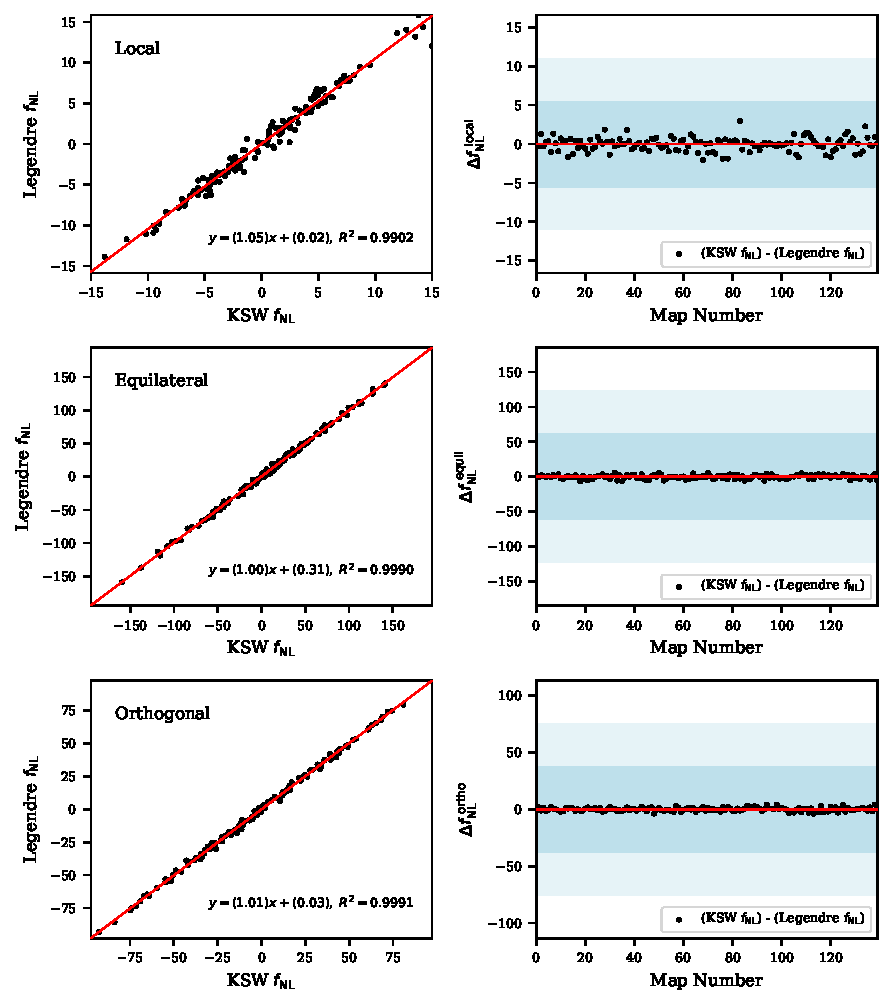
\includegraphics[width=\textwidth]{map_by_map_Legendre_KSW.pdf}
	\caption{Map-by-map comparison of $f_{NL}$ estimates for standard templates, evaluated using each of the KSW and Legendre basis sets. Planck 2018 CMB map and 140 FFP10 simulations have been used, each representing a single point on the scatter plot shown left. Details of the linear best-fit to data (red dashed) is annotated below. On the right hand side shows a plot of $f_{NL}$ values for each map. In the ideal case where the two basis sets yield identical results, we should see all the points on $y=x$ for the left plot, and exactly overlapping graphs for the right. For more information on  each of the three theoretical templates used, see e.g., \cite{PlanckCollaboration2013}.}
	\label{fig:map_by_map_Legendre_KSW}
\end{figure}

We see that results from the two different sets of basis are in good agreement. The $R$-squared value of the linear fit is greater than $0.99$ for Local, and $0.999$ for Equilateral and Orthogonal shapes. The intercept and sample mean are also near zero. We do not find any systematic discrepancies across the shapes from individual map estimates either.

The fact that results from the KSW and Legendre basis are consistent validates multiple aspects of our pipeline. First of all, we can deduce that the Legendre basis expansion (\ref{eqn:basis_expansion}) accurately represents the bispectrum shapes of interest, especially since the KSW basis is designed to be exact for the three standard shapes. Having $p_{max}=30$ modes is more than sufficient. Figure \ref{fig:map_by_map_Legendre_30_29} explicitly compares results obtained from Legendre bases with $p_{max}=29$ and $30$, while keeping everything else the same. The two results show absolute agreement, the largest of errors less than $O(10^{-5})$. This further confirms that our expansion using Legendre polynomials have completely converged.

\begin{figure}[htbp!] 
	\centering    
	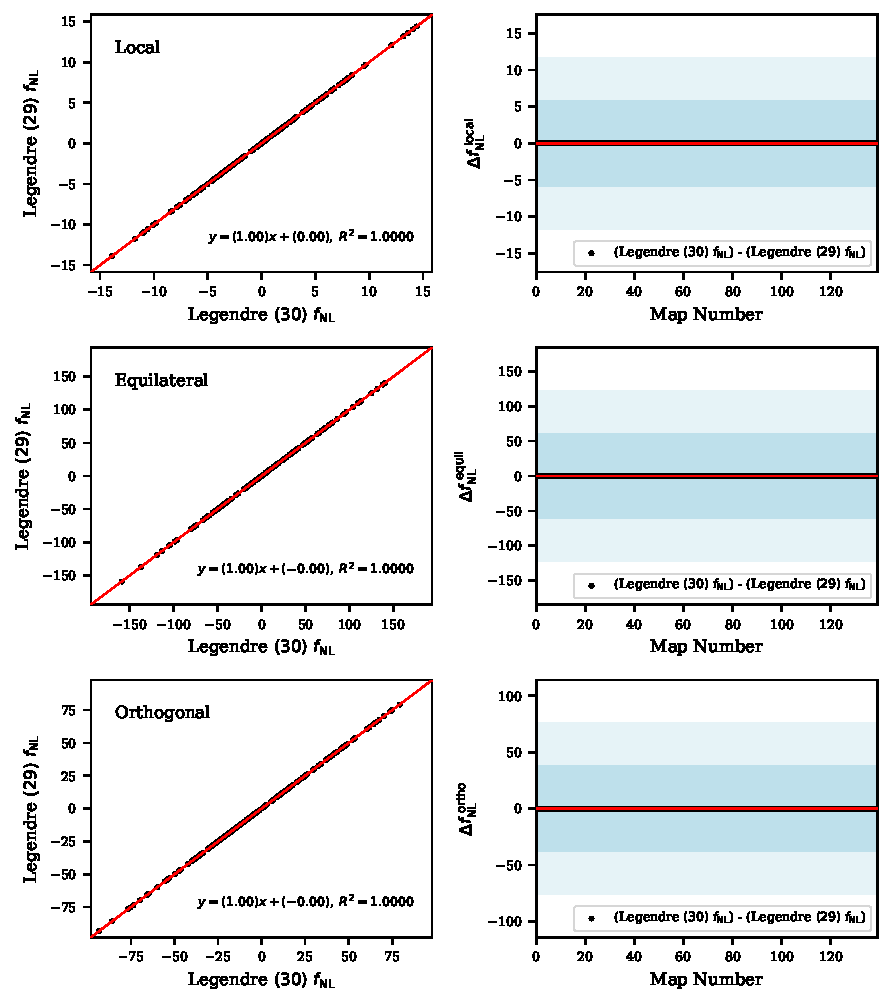
\includegraphics[width=\textwidth]{map_by_map_Legendre_30_29.pdf}
	\caption{Map-by-map comparison of $f_{NL}$ estimates for standard templates using the Legendre basis with different number of modes: $p_{max}=29$ and $30$. The two results agree with error less than $O(10^{-5})$, as can be seen from the scatter plots (left) and map-by-map plots (right). This confirms that our expansion using Legendre polynomials has completely converged for these bispectrum shapes.}
	\label{fig:map_by_map_Legendre_30_29}
\end{figure}

Secondly, we validated the accuracy of linear term and lensing-ISW bias calculations through sample mean of $f_{NL}$ estimates from lensed simulations. When we exclude either of the two, we find the sample mean to be far from zero. The error is especially large for Local template. Linear term accounts for the anisotropy introduced by masking parts of the observed sky. The squeezed limit contribution to bispectrum comes from couplings between a pair of small-scale modes and a large-scale one, making it more susceptible to bias from partial coverage. Presence of sky masks therefore offsets the $f_{NL}$ estimates from Local shape which has large squeezed limit. Lensing-ISW bias is also the largest in squeezed configurations and affects Local $f_{NL}$. The fact that our lensed Gaussian simulations have $f_{NL}$s fluctuate around $0$ validates our bias subtractions.

Lastly, we check that CMB-BEst accurately preserves optimality of the CMB bispectrum estimator. In the weak non-Gaussian limit, the estimator (\ref{eqn:bispectrum_estimator_standard}) saturates the Cramer-Rao bound. Its expected variance is the lowest amongst all possible unbiased bispectrum estimators of $f_{NL}$. Heuristically speaking, the estimator extracts as much information about non-Gaussianity as possible from the CMB bispectrum . As we discussed in Chapter \ref{chapter:CMB_state-4_forecast}, this bound only depends on the Fisher information determined from normalisation; $Var[\hat{f}_{NL}]=F^{-1}=6/N$. We refer to this value as the \textit{theoretical} variance (the best possible from theory). Meanwhile, individual $f_{NL}$ estimates from simulated maps and independent and normally distributed. Sample variance obtained from $N_{sims}$ simulations should therefore approach the theoretical variance as $N_{sims}\rightarrow\infty$. Table \ref{table:trio_sample_and_theory_variances} summarises calculated values of the two types of variances discussed.

\begin{table}[h]
	\caption{Comparison of the sample and theoretical variances obtained from $f_{NL}$ estimates of standard shapes, computed using each of the KSW and Legendre basis sets. Sample variances are within $1\sigma$ interval from theoretical values assuming that the 140 individual $f_{NL}$'s from simulated maps are normally distributed. This is statistically consistent with optimality of our bispectrum estimator.}
	\centering
	\label{table:trio_sample_and_theory_variances}
	\renewcommand{\arraystretch}{1.5} 
	\begin{tabular}{llccc}
		\toprule
		Template & Basis & Sample Variance &  Theoretical Variance &  (Sample)/(Theory) \\
		\midrule
		\multirow{2}{*}{Local} & KSW &  5.5 &       5.3 &               1.04 \\
		& Legendre &             5.9 &                  5.7 &               1.04 \\
		\multirow{2}{*}{Equilateral} & KSW &            61.2 &                 67.7 &               0.90 \\
		& Legendre &            61.7 &                 67.7 &               0.91 \\
		\multirow{2}{*}{Orthogonal} & KSW &            37.7 &                 33.7 &               1.12 \\
		& Legendre &            38.0 &                 33.9 &               1.12 \\
		\bottomrule
	\end{tabular}
\end{table}

Note that the numbers do not match up exactly between sample and theoretical variances. The estimator for sample variance $\hat{S}^2 = (\sum_i (f^{(i)}_{NL})^2 )/N_{sims}$ follows chi-squared distribution with $N_{sims}-1$ degrees of freedom under our assumptions. Standard deviation corresponding to the (normalised) distribution equals $\sqrt{2/(N_{sims}-1)}$, which is $\approx 0.12$ for $N_{sims}=140$. It is therefore not surprising to see our sample variances differ up to $12\%$ from the theoretical ones.

We performed further checks to ensure that this discrepancy is due to statistical fluctuations rather than systematic errors. The ratio between sample and theoretical variances remained nearly constant across the KSW and Legendre basis from CMB-BEst, as well as Planck's Modal pipeline on the same set of simulated maps. Meanwhile, sample variances evaluated from independent sets of simulations do fluctuate around the theoretical value. A closer check has been done for each of the mode sets $(p_1,p_2,p_3)$ in the Legendre basis. The decomposition coefficient $\alpha$ is set to be 1 at $(p_1,p_2,p_3)$ and its permutations, while vanishing everywhere else. Substituting into \eqref{eqn:fNL_from_betas} and \eqref{eqn:normlisation_from_gamma}, we get
\begin{align}
	f_{NL}^{(i)} &= \frac{1}{N} \left[ \left( \beta^{cub,(i)}_{p_1 p_2 p_3} - 3 \beta^{lin,(i)}_{p_1 p_2 p_3} \right) + \text{5 cyc.} \right], \\
	N &= 6\left( \Gamma_{p_1 p_2 p_3, p_1 p_2 p_3} + \Gamma_{p_1 p_2 p_3, p_1 p_3 p_2} + \cdots + \Gamma_{p_1 p_2 p_3, p_3 p_2 p_1} \right).
\end{align}
Here we assumed that $p_1,p_2,p_3$ are distinct for convenience. Corresponding sample and theoretical variances have been compared for each of the modes. Overall, they are found to be statistically consistent as before.

% Optional: could include a historgram plot for (sample var)/(theory var) calculated for each of the modes (p1,p2,p3) in Legendre basis. p_max = 30 would make the plot look sufficiently smooth...

While Figure \ref{fig:map_by_map_Legendre_KSW} shows excellent agreement between results from the KSW and Legendre basis sets overall, there are small but noticeable scatters in the plot for Local shape. The slope of linear best fit is also slightly above 1, meaning that $f_{NL}$ estimates from Legendre routine tend to vary 5\% more than the KSW ones. Larger variance means less information extracted. Our first hypothesis was that Legendre polynomials are losing small fraction of information due to their fixed $k$ range in their definition ($\ref{eqn:Legendre_basis_no_inv_k}$). We test this by increasing the range by changing $k_{max}/k_{min} = 1000$ to $2000$. The results are shown in Figure \ref{fig:map_by_map_Legendre_KSW_k_ratio_2000}.

\begin{figure}[htbp!] 
	\centering    
	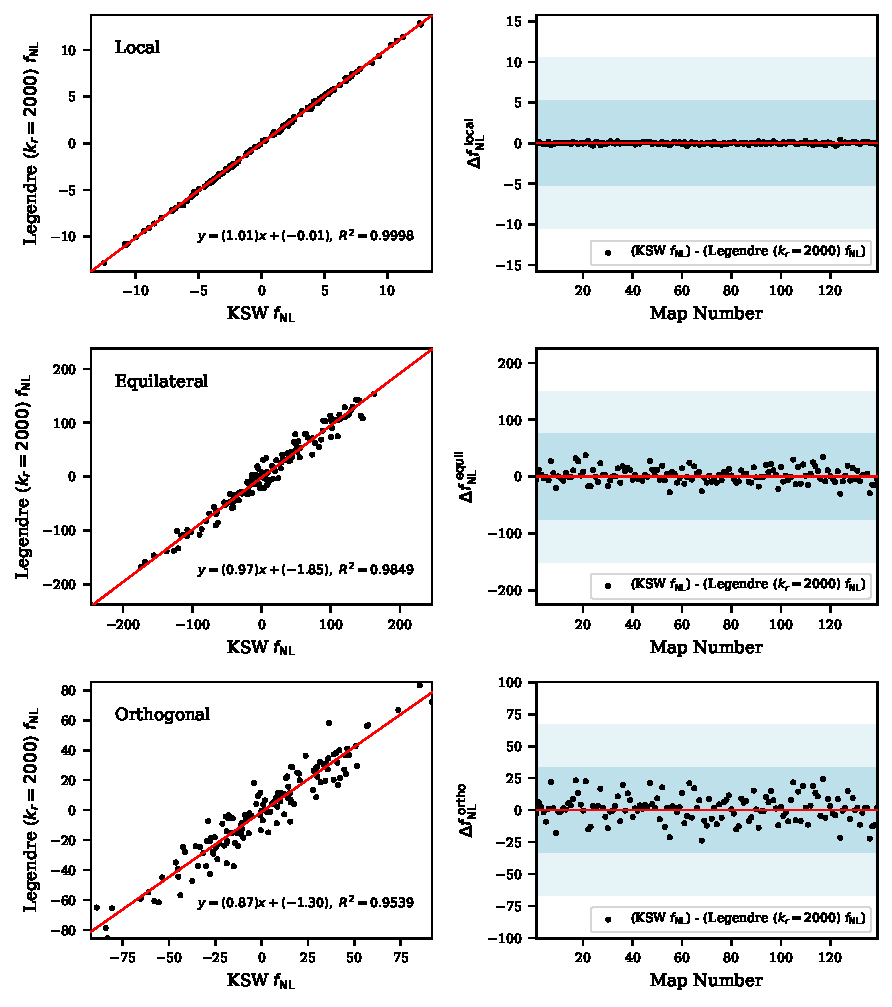
\includegraphics[width=\textwidth]{map_by_map_Legendre_KSW_k_ratio_2000.pdf}
	\caption{Map-by-map comparison of $f_{NL}$ estimates for standard templates from the KSW and Legendre basis sets, similar to Figure \ref{fig:map_by_map_Legendre_KSW}. Here, the Legendre basis has a wider $k$ domain: $k_{max}/k_{min} = 2000$ instead of the usual $1000$. Number of modes ($p_{max}$) has been reduced to $10$ instead of $30$ for simplicity. We see that additional information from large scales (low $k$) fixes the small scatter present in $f_{NL}^{local}$ of the previous plot.}
	\label{fig:map_by_map_Legendre_KSW_k_ratio_2000}
\end{figure}

Our main focus of this figure lies on Local template results. Estimates from the KSW and Legendre basis sets match almost perfectly now. When altering the ratio $k_{max}/k_{min}$, we fixed the $k_{max}$ and lowered $k_{min}$. Including more small-$k$, or large scale modes provides extra information in the bispectrum. Local shape is especially affected by this, since squeezed configurations including one of these extra large scale modes have a more significant contribution to the total estimate. Also note that $k_{max} / k_{min} = 2000$ is comfortably larger than the equivalent ratio in harmonic space $l_{max} / l_{min} = 2500 / 2$.

Despite the improvements in squeezed limit and local template, we may not simply set $k_{max} / k_{min} = 2000$ as default because it hurts convergence in other shapes of interest. As can be seen from the Equilateral and Orthogonal plots in Figure \ref{fig:map_by_map_Legendre_KSW_k_ratio_2000}, newer estimates of $f_{NL}$ are less accurate for shapes other than Local. The fact that $p_{max}=10$ here rather than $30$ is one of the main causes of the drop in precision, but having smaller $k$ values within Legendre polynomials' domain also has a negative impact. Shapes with inverse $k$ scaling vary more dramatically when $k$ is small and tends to be harder to expand in terms of Legendre polynomials.

For the final check of internal consistency, we inspect how each point in the line of sight integral ($r$) contributes to $f_{NL}$ estimates. CMB-BEst's formalism makes it straightforward to plot the $r$ integrand since the integral is done at the very last. Figure \ref{fig:trio_r_dependence} shows plots of $f_{NL}$ contributions from different sources and for the three standard bispectrum templates. Shaded in light blue are the $1\sigma$ regions obtained from 140 simulations for each point in $r$.

\begin{figure}[htbp!] 
	\centering    
	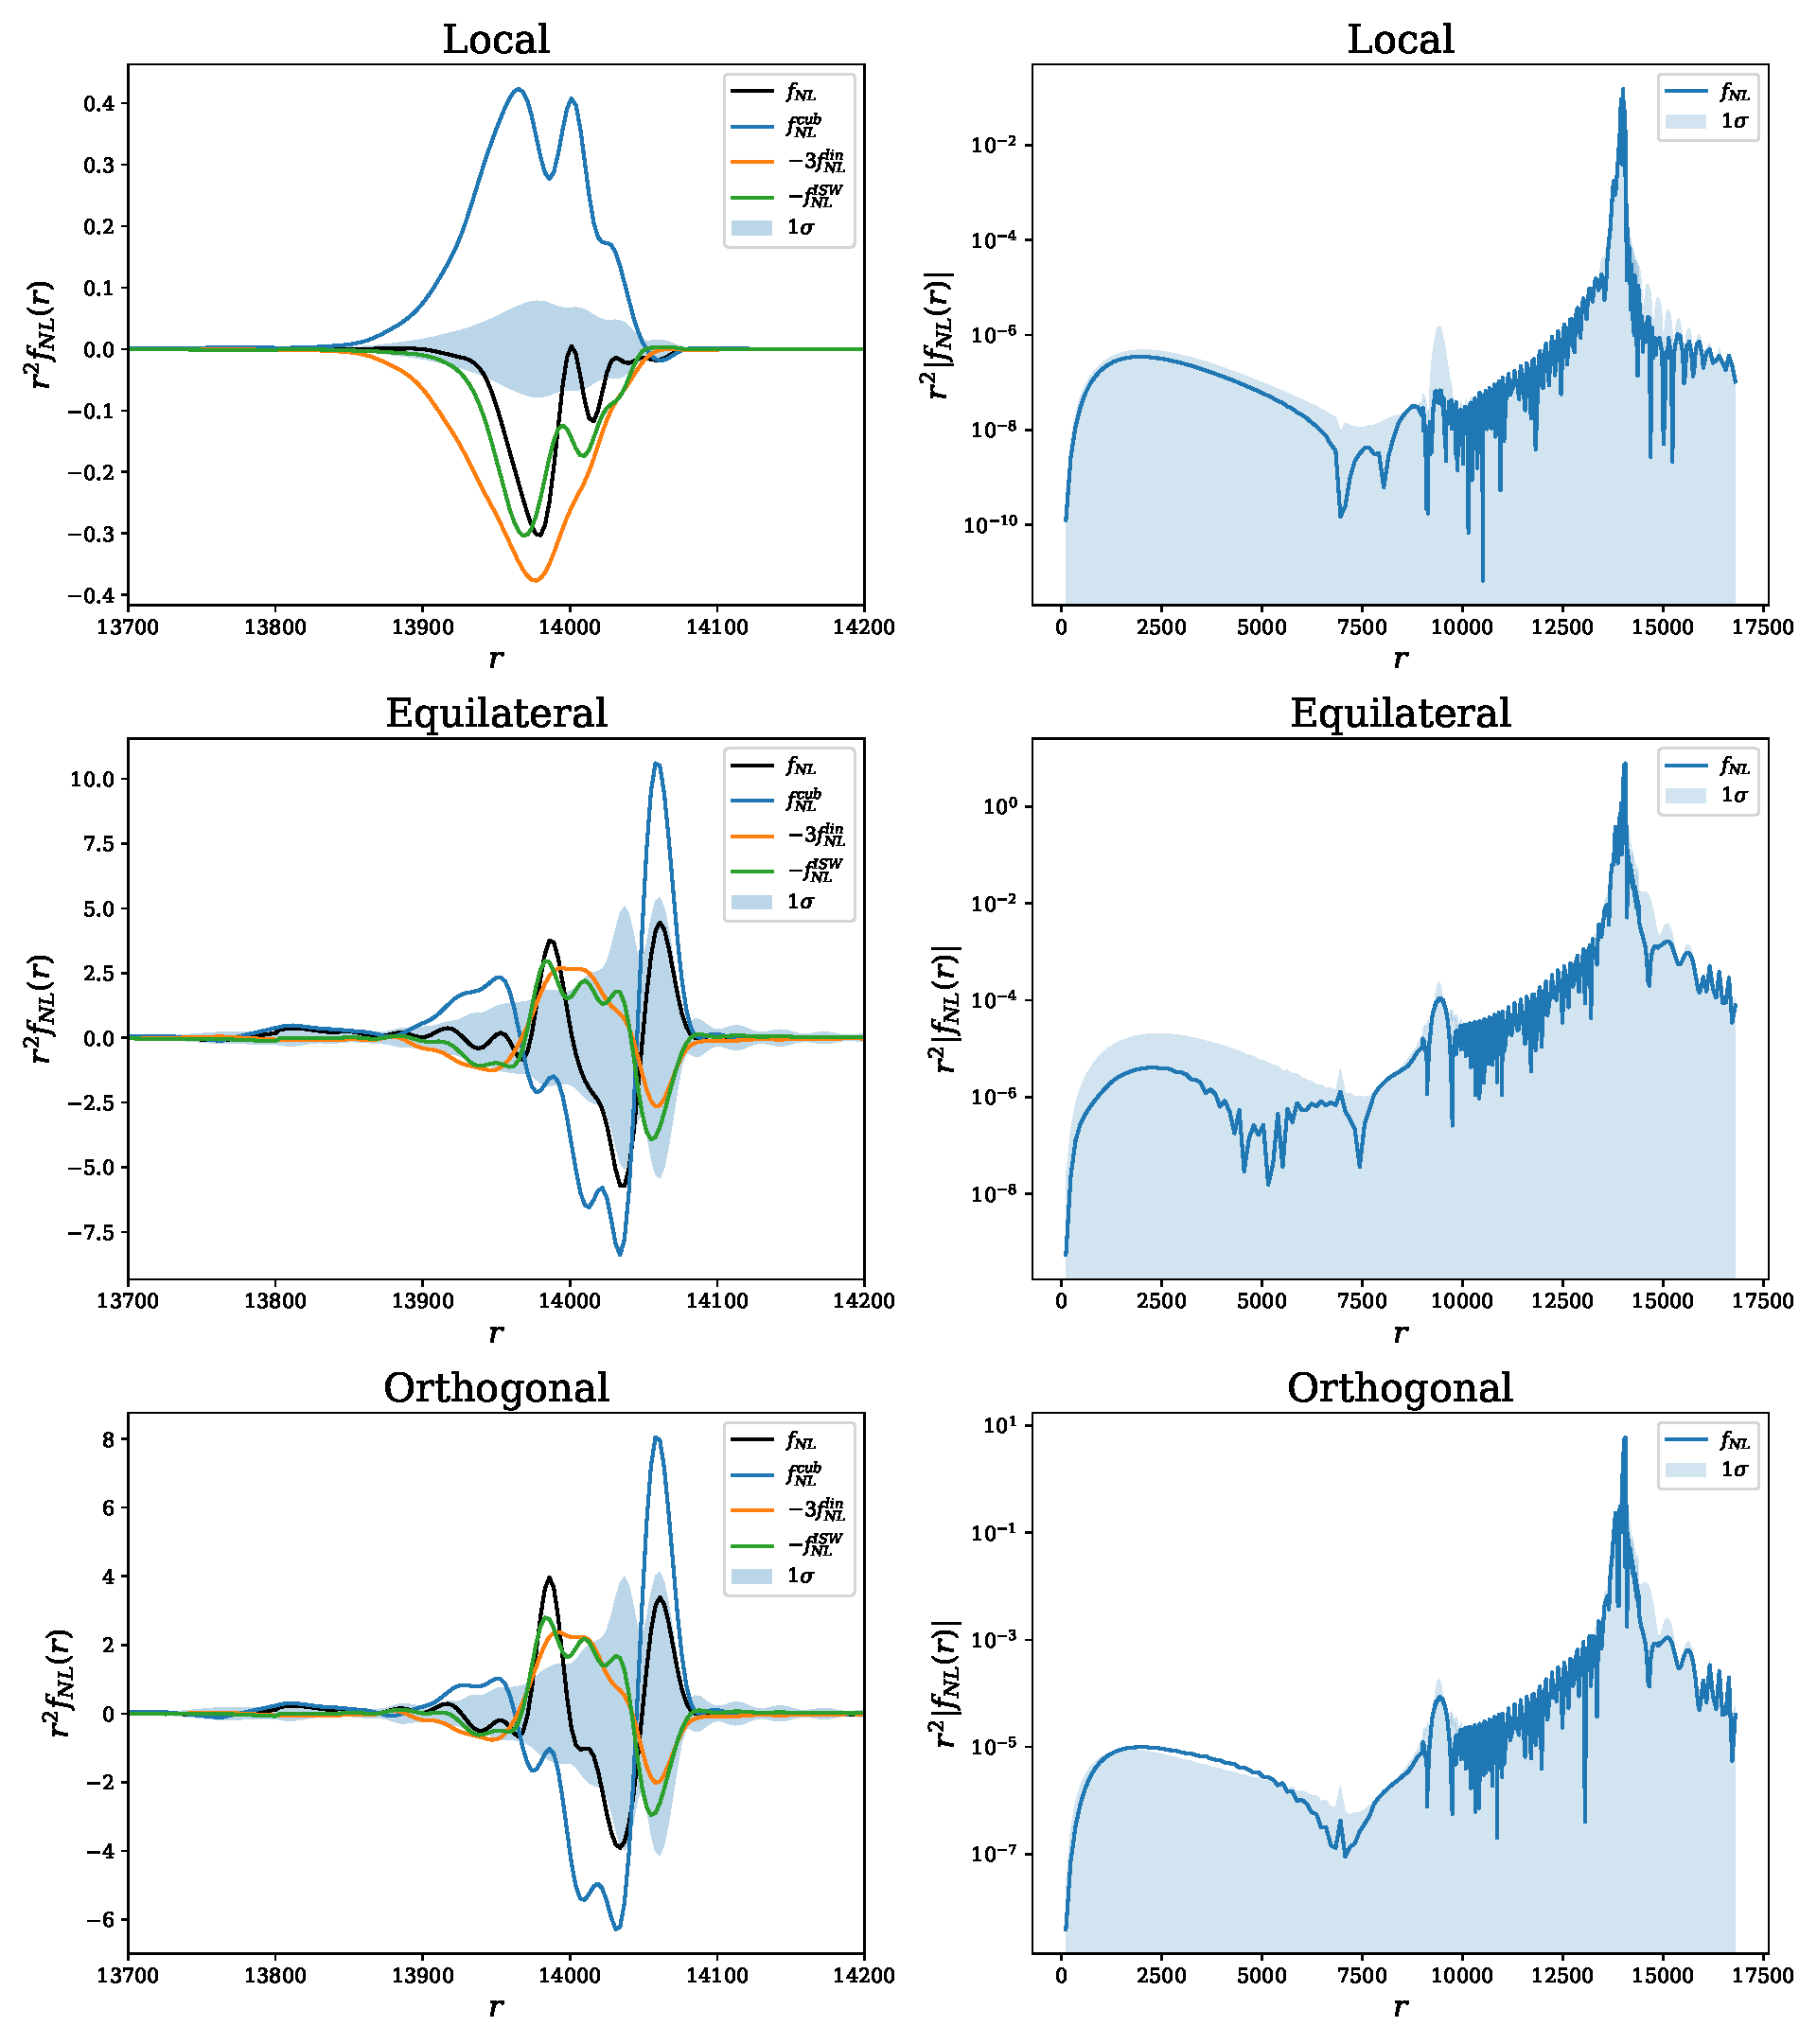
\includegraphics[width=\textwidth]{trio_r_dependence.pdf}
	\caption{Contributions to the total $f_{NL}$ from each point in the line-of-sight integral over $r$ for standard templates. On the left hand side, we plot contributions from the cubic, linear, and lensing-ISW bias, as well as the total $f_{NL}$. Shown in blue is the $1\sigma$ interval obtained from corresponding terms in 140 FFP10 Gaussian simulations. We focus on the $r$ interval around recombination where most of the signal comes from. Plots on the right hand side show $f_{NL}$ contributions over the whole $r$ range in log scale. ISW effect, reionisation, and recombination are responsible for the three most noticeable peaks in all three plots.}
	\label{fig:trio_r_dependence}
\end{figure}

As illustrated in plots on the right hand side of Figure \ref{fig:trio_r_dependence}, the vast majority of signal comes from recombination around $r = 14,000$Mpc. In fact, its contribution is dominant enough so that neglecting signal from everywhere else would still be a good approximation. CMB-BEst uses an adaptive $r$ grid which is denser around recombination, following the works of \cite{Smith2011}. Other small but notable contributions to the total estimate come from reionisation ($r \sim 10,000$Mpc) and ISW effect ($r < 5,000$Mpc).

Zooming in on an interval around recombination, significant contributions from the cubic term to $f_{NL}$ of Local template is rather prominent (upper left of Figure \ref{fig:trio_r_dependence}). The signal is sufficiently larger than the expected random fluctuations evaluated from Gaussian simulations, which could be hinting non-zero primordial non-Gaussianity. However, contributions from the linear term (shown orange) completely counterbalances it, bringing the total down to values consistent with zero. This again validates accuracy of our methodology; bias to $f_{NL}$ generated from anisotropic sky masks are precisely subtracted off using the linear terms.

We do not find any statistically significant signal across the whole $r$ range otherwise, especially when taking look-elsewhere effect into account. It is not meaningful to find a couple 3-4$\sigma$ values when the other 500 points are simply disregarded. If we detect primordial non-Gaussianity in the future, however, then these plots of $f_{NL}$ contributions for each $r$ will provide valuable insights on where the signal comes from.

% Write about convergecne? 
%- Convergence epsilon definition
%- Standard templates convergence epsilons
%- Legendre - constant feature models part. Correlation matrix


\subsection{Consistency with Planck} \label{section:consistency_with_Planck}

In the last section, we demonstrated how the integrity of CMB-BEst was validated. The next set of validations involves comparing it against other existing codes for CMB bispectrum estimation.

We test primordial non-Gaussianity constraints on Local, Equilateral and Orthogonal templates against the Planck 2018 analysis \cite{PlanckCollaboration2018}. Two sets of basis functions, KSW and Legendre, have been used to compute $f_{NL}$ from the foreground-cleaned CMB map included in the final data release. We choose SMICA as the main component separation method since they were shown to be the most reliable and robust for Planck bispectrum analysis \cite{PlanckCollaboration2013ComponentSeparation, PlanckCollaboration2013,PlanckCollaboration2015,PlanckCollaboration2018}. Table \ref{table:trio_fNL_comparison_with_planck} summarises the constraints obtained, together with the quoted results from Planck team's own KSW estimator and Modal 2 pipeline.

\begin{table}[h]
	\caption{Constraints on $f_{NL}$ for the standard shapes from the KSW and Legendre basis of CMB-BEst, in comparison with the Planck 2018 analysis \cite{PlanckCollaboration2018}. Only the temperature data from the SMICA foreground-cleaned map and FFP10 simulations were used for the analysis. Values shown are after the lensing bias subtraction, with uncertainties at 68\% CL.}
	\centering
	\label{table:trio_fNL_comparison_with_planck}
	\renewcommand{\arraystretch}{1.5} 
	\begin{tabular}{lcccc}
		\toprule
		& \multicolumn{2}{c}{CMB-BEst} & \multicolumn{2}{c}{Planck 2018} \\ \cmidrule(lr){2-3} \cmidrule(lr){4-5}
		Shape & KSW &  Legendre &  KSW &  Modal \\
		\midrule
		
		Local & $-2.2 \;\pm\; 5.5$ & $-2.0 \;\pm\; 5.9$ & $-0.5 \;\pm\; 5.6$ & $-0.6 \;\pm\; 6.4$ \\
		Equilateral & $17 \;\pm\; 61$ & $15 \;\pm\; 62$ & $7 \;\pm\; 66$ & $34 \;\pm\; 67$ \\
		Orthogonal & $-7 \;\pm\; 38$ & $-9 \;\pm\; 38$ & $-15 \;\pm\; 36$ & $-26 \;\pm\; 43$ \\
		\bottomrule
	\end{tabular}
\end{table}

Note that while the constraints from CMB-BEst are largely consistent with Planck 2018 results, there are up to $0.3\sigma$ discrepancies. However, there are variations around this level within the estimates from different pipelines of Planck as well. Equilateral constraints from Planck's own KSW and Modal estimators shown here, for example, differ by $\approx 0.4\sigma$. Similar amount of fluctuations can be found in the full result shown in \cite{PlanckCollaboration2018}. Even though in an ideal world they should match exactly across different approaches as long as same dataset is used, statistical significance of the individual $f_{NL}$'s is not largely affected by such variations.

We invested significant proportion of our time investigating this error. Here we discuss three potential sources which might account for the discrepancies. First of all, human error during implementation and estimation process should not be neglected. Bispectrum analysis is complex and computationally expensive. Implementing it often involves writing a long and heavily optimised code. During development and testing stages, we found and fixed many mistakes in our $10,000+$ lines of \textsc{C} code. Various unit tests were performed in the process to test individual sections of the code: basis expansion, projection to the $l$ space, SHTs, parallelisation, and more. Internal consistency checks were then used to verify integrity of the combined pipeline. Planck team also went on lengths to validate and cross-check different methods \cite{PlanckCollaboration2013}. It therefore seems unlikely that simple mistakes are causing the gap in results.

Next source of error we studied is the parameter set. Cosmological parameters we used for constraints in Table \ref{table:trio_fNL_comparison_with_planck} are identical to those of Planck Modal pipeline. Small changes in cosmological parameters are also shown to have little effect on $f_{NL}$ \cite{PlanckCollaboration2015,PlanckCollaboration2018}. One major difference however, is the number of Gaussian simulations used. We include 140 simulated maps while Modal has about 300. This number is mainly restricted by computational resources required for the large Legendre basis in CMB-BEst. While we found 140 to be sufficient for most cases, sample variance may cause some fluctuations in the linear term and error bar. A rough estimate for sampling error is $\sim \sqrt{2/N_{sims}} \approx 0.12$, as calculated in the previous section. Other than $N_{sims}$, more internal parameters such as the grid density of discretised arrays have also been checked to yield consistent results when varied. 

We are left with systematic errors as potential causes for discrepancies. The most significant bias to $f_{NL}$ constraints is the lensing-ISW bias discussed in Section \ref{section:other_sources_of_non_gaussianity}. Table \ref{table:trio_lensing_bias_comparison_with_planck} shows biases from the lensing bispectrum \cite{Lewis2011lensing} for both CMB-BEst and Planck 2018 analysis. The numbers vary but are consistent overall. Map-by-map comparison of constraints from the Legendre basis and Modal are shown in Figure \ref{fig:map_by_map_Legendre_Modal}. 

\begin{table}[h]
	\caption{Bias to $f_{NL}$ of standard shapes originating from the lensing bispectrum. We compare CMB-BEst's two different basis sets and the Planck 2018 analysis \cite{PlanckCollaboration2018}, using SMICA map and FFP10 simulations. }
	\centering
	\label{table:trio_lensing_bias_comparison_with_planck}
	\renewcommand{\arraystretch}{1.5} 
	\begin{tabular}{lcccc}
		\toprule
		& \multicolumn{2}{c}{CMB-BEst} & \multicolumn{2}{c}{Planck 2018} \\ \cmidrule(lr){2-3} \cmidrule(lr){4-5}
		Shape & KSW &  Legendre &  KSW &  Modal \\
		\midrule
		
		Local & $7.5$ & $8.2$ & $7.3$ & $6.9$ \\
		Equilateral & $-0.7$ & $-0.6$ & $-0.7$ & $4.0$\\
		Orthogonal & $-22$ & $-22$ & $-23$ & $-25$ \\
		\bottomrule
	\end{tabular}
\end{table}

\begin{figure}[htbp!] 
	\centering    
	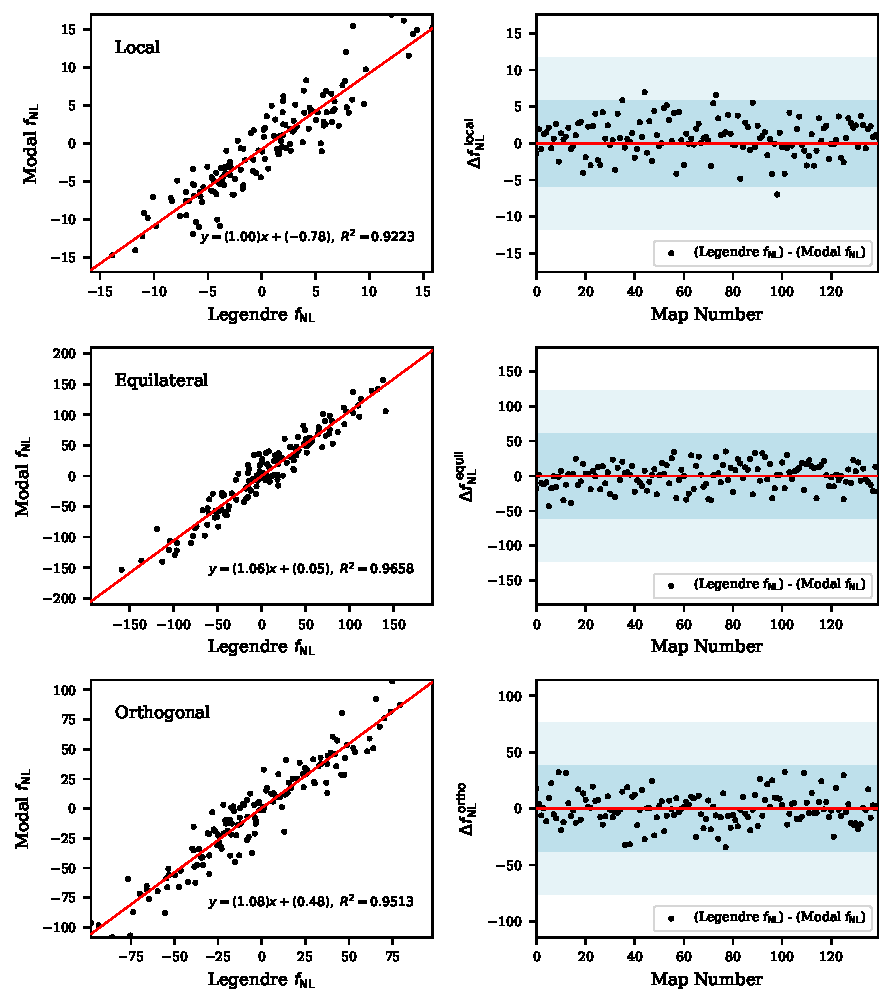
\includegraphics[width=\textwidth]{map_by_map_Legendre_Modal.pdf}
	\caption{Map-by-map comparison of the $f_{NL}$ estimates obtained from CMB-BEst's Legendre basis set against the Modal estimator results for Planck 2018 analysis \cite{PlanckCollaboration2018}. The first 140 FFP10 simulations are used. On the left hand side are scatter plots where each simulation is represented by a point according to $f_{NL}$ estimates of standard templates. Their linear best fit lines are shown in dashed red. Results from the two routines are shown map by map on the right hand side. Overall, CMB-BEst and Modal are in good agreement, without any significant systematic errors.}
	\label{fig:map_by_map_Legendre_Modal}
\end{figure}

Out of the three templates, local shape shows the largest scatter between constraints. Comparing $f_{NL}$'s of simulated maps from CMB-BEst and Modal, we find correlation of 0.916. The intercept value of $0.78$ in the linear fit is mainly due to sample mean present in Modal. Legendre's sample mean is $0.069$ for Local, while Modal has $-0.698$. Otherwise, the difference between two pipelines are distributed such that its sample standard deviation equals $2.5$, skewness is $-0.14$, and kurtosis is $0.19$. Having small skewness and kurtosis less than $1$ implies that the distribution is close to univariate normal, consistent with random fluctuations. Similarly, we do not find any significant systematic error from Equilateral and Orthogonal shapes either.

Having not found a clear source of error, we conclude that the small gaps between the $f_{NL}$ estimates in Table \ref{table:trio_fNL_comparison_with_planck} mainly come from differences in methodology and are consistent with random fluctuations.

We now move on to constraining models with oscillations. The simplest template for oscillatory models is the feature model studied in Chapter \ref{chapter:CMB_state-4_forecast}. We use a template shape function of form $S^\text{feat}(k_1,k_2,k_3) = \sin(\omega (k_1 + k_2 + k_3) + \phi)$. Figure \ref{fig:sine_template_frequency_Legendre_Modal} shows $f_{NL}$ constraints obtained from the Legendre basis and compares them with Modal results from Planck 2018 analysis. The `phase' $\phi$ is set to zero, while oscillation `frequency' $\omega$ was varied from $10$ Mpc to $350$ Mpc. We follow \cite{Fergusson2015a} and increase $\omega$ in steps of $10$, so that correlation between shapes with different $\omega$ is kept low.

\begin{figure}[htbp!] 
	\centering    
	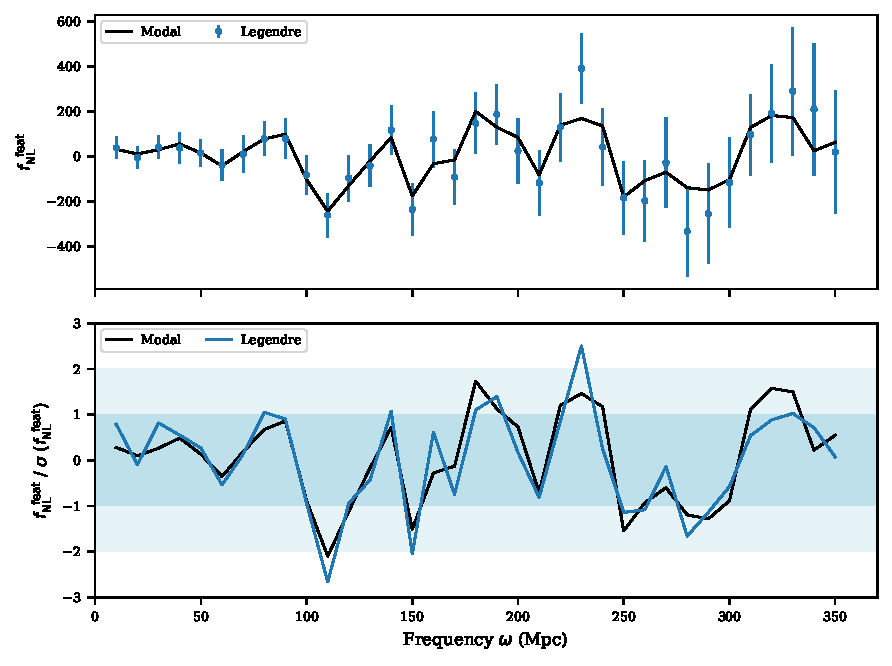
\includegraphics[width=\textwidth]{sine_template_frequency_Legendre_Modal.pdf}
	\caption{Estimated $f_{NL}$'s for feature models with shape $S(k_1,k_2,k_3) = \sin(\omega (k_1 + k_2 + k_3)$, obtained using the Legendre basis with (blue) and Planck's Modal (black). Left: direct comparison of $f_{NL}$ for different values of $\omega$. Error bars indicate the expected standard deviation in the estimator, calculated using 140 Gaussian simulations. Right: measured signal-to-noise $f_{NL}/\sigma$, again for a range of $\omega$ values. Shaded in blue are the $1\sigma$ and $2\sigma$ levels. We see that the two approaches yield coherent estimates overall.}
	\label{fig:sine_template_frequency_Legendre_Modal}
\end{figure}

The Legendre basis accurately expands the feature model template using Legendre polynomials via basis expansion outlined in (\ref{eqn:basis_expansion}). Estimates from the two methods, CMB-BEst's Legendre and Planck's Modal, are mostly compatible. The most notable difference is at $\omega=230$Mpc where $f_{NL}$ from Legendre is more than $1\sigma$ larger compared to Modal. Even though it is interesting that the new estimate now passes the $2\sigma$ threshold, having one such point out of 35 shown here has less statistical significance.

Both Legendre and Modal approaches involve expanding the shape function with respect to a polynomial basis. Polynomials are versatile but has limited resolution for oscillatory signals; it cannot resolve shape with number of oscillations greater than the maximum degree of polynomials ($p_{max}$ here). For the Legendre basis with $k$ range $[2.09\times 10^{-4}, 2.09\times 10^{-1}]\text{Mpc}^{-1}$ and $p_{max}=30$, frequencies greater than $\pi p_{max} / (k_{max} - k_{min}) \approx 436$Mpc are unresolvable. In reality, numerics start to break before this value. We do not have a reference analytic value for true $f_{NL}$s, but evaluating correlations between shapes is effective for checking our numerics.

\begin{figure}[htbp!] 
	\centering    
	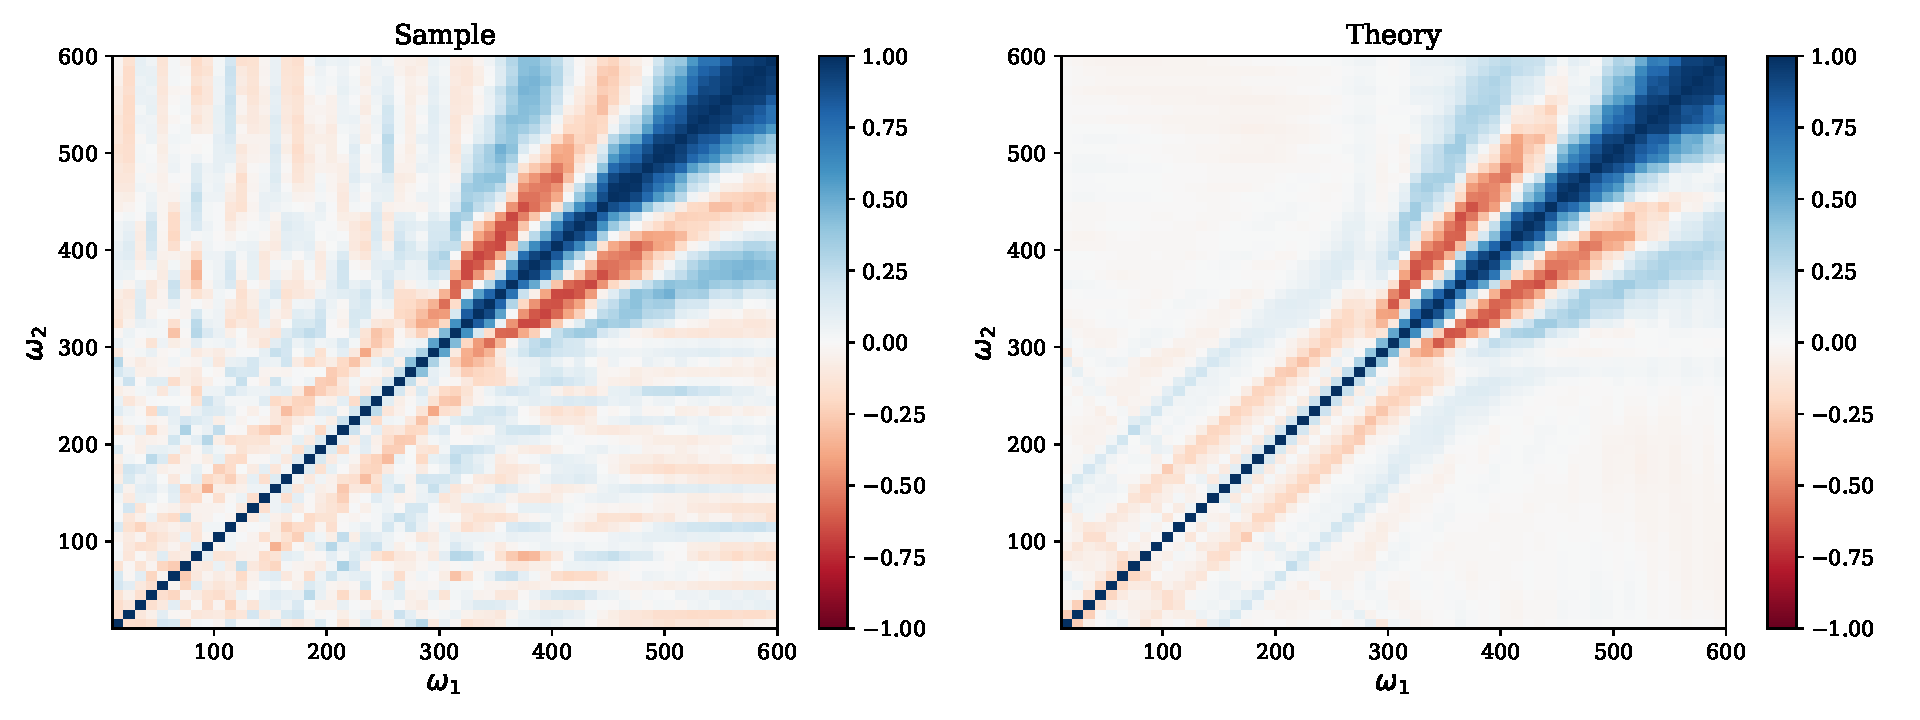
\includegraphics[width=\textwidth]{sine_template_correlations_new.pdf}
	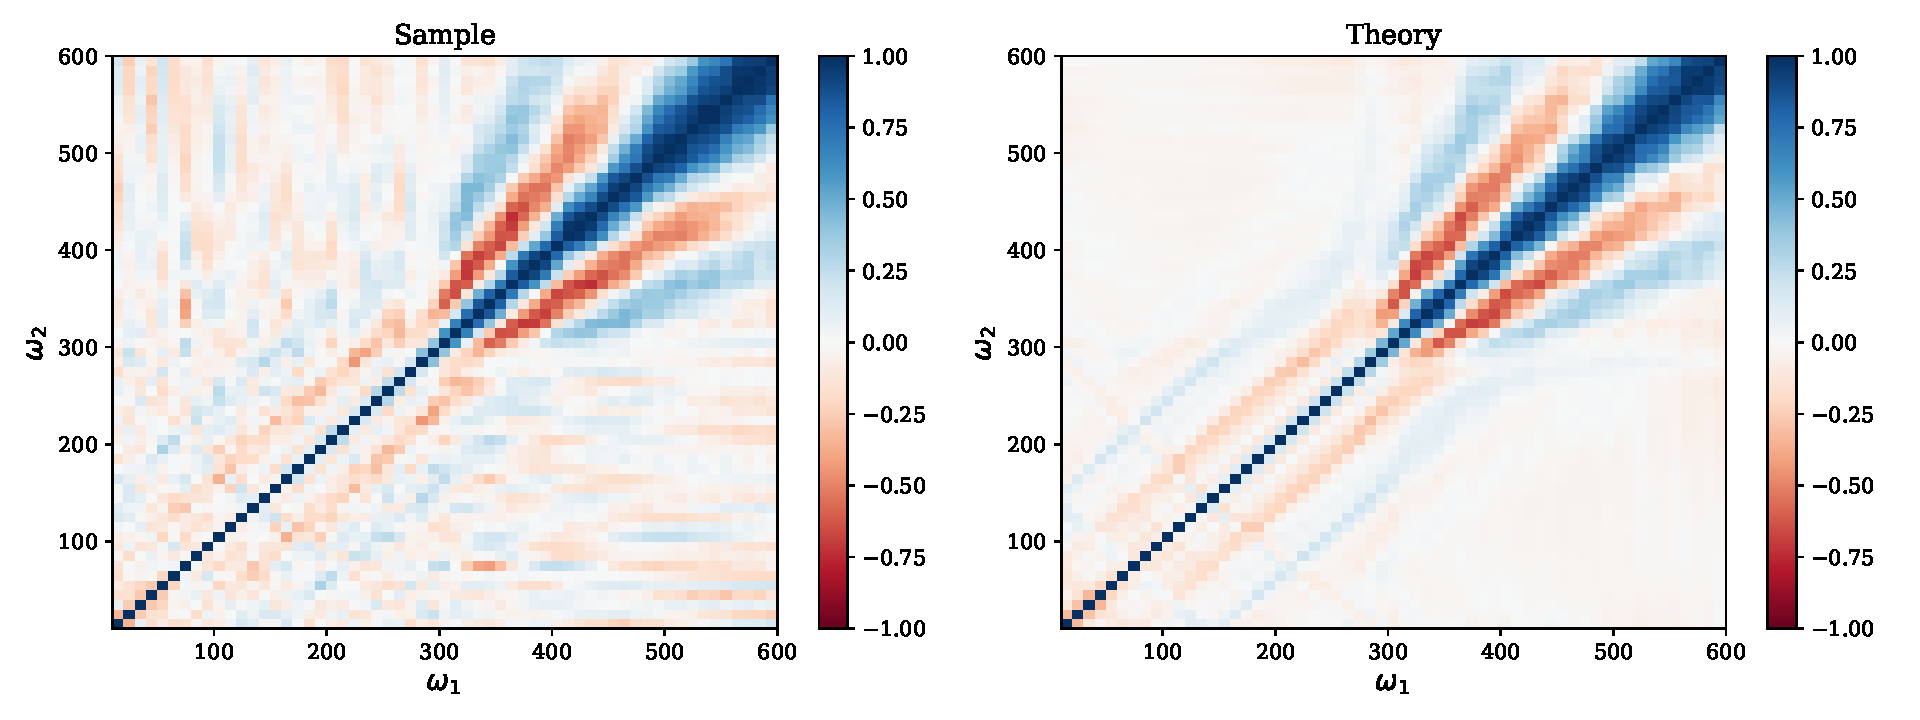
\includegraphics[width=\textwidth]{cosine_template_correlations_new.pdf}
	\caption{Correlations between feature model templates $S(k_1,k_2,k_3)=\sin(\omega (k_1 + k_2 + k_3) + \phi)$ with different $\omega$ values, for $\phi = 0$ (top two) and $\phi = \pi/2$ (bottom two). Results are from Legendre basis. `Sample' correlations are obtained from the $f_{NL}$ estimates from 140 Gaussian simulations, while `theory' correlations come from the inner product induced by $\Gamma_{p_1 p_2 p_3, p_1 p_2 p_3}$ matrix in (\ref{def:gamma}). Large non-diagonal correlations appear around $\omega \approx 300$, after which oscillations in the shape are no longer resolved by polynomials of degree up to $p_max$.}
	\label{fig:feature_template_correlations}
\end{figure}

Figure \ref{fig:feature_template_correlations} shows correlations between $f_{NL}$s from feature models with different frequency $\omega$s. The plots show correlation between $f_{NL}$ estimates from 140 FFP10 Gaussian simulations (`sample'), together with the one evaluated using our `late-time' inner product ('theoretical') given by
\begin{align}
	\left< b^{(i)}, b^{(j)} \right> &= \sum_{l_j} \frac{h^2_{l_1 l_2 l_3} b^{(i)}_{l_1 l_2 l_3} b^{(j)}_{l_1 l_2 l_3}}{C_{l_1} C_{l_2} C_{l_3}}  \\
	&= \sum_{p_j p'_j} \alpha^{(i)}_{p_1 p_2 p_3} \alpha^{(j)}_{p'_1 p'_2 p'_3} \sum_{l_j} \frac{h^2_{l_1 l_2 l_3} (b^{(i)}_{p_1 p_2 p_3})_{l_1 l_2 l_3} (b^{(j)}_{p'_1 p'_2 p'_3})_{l_1 l_2 l_3}}{C_{l_1} C_{l_2} C_{l_3}} \\
	&= \sum_{p_j p'_j} \alpha^{(i)}_{p_1 p_2 p_3} \alpha^{(j)}_{p'_1 p'_2 p'_3} \Gamma_{p_1 p_2 p_3, p'_1 p'_2 p'_3} \\
	&= \vv{\alpha^{(i)}} \; \Gamma \; \vv{\alpha^{(j)}}, \label{eqn:late_time_inner_product}
\end{align}
where $\Gamma$ is defined in (\ref{def:gamma}). In the limit $N_{sims} \rightarrow \infty$, the sample correlation can be shown to approach the theoretical value in the weakly non-Gaussian limit. We see from Figure \ref{fig:feature_template_correlations} that they indeed display the same qualitative behaviour for $N_{sims}=140$.

The templates with $\omega < 300$ are highly uncorrelated with each other, as can be seen from small non-diagonal elements. Noticeable correlations on lines $\omega_2 = \omega_1 \pm c$ for $c = 70, 140$ arise from resonance between oscillations and transfer functions at the Baryonic Acoustic Oscillation (BAO) scale, as we observed in Figure \ref{insight feature plot}. Faint lines can also be found near $\omega_2 = -\omega_1 + c, \;\; c = 70,140,210,\cdots$ for similar reasons.

When $\omega > 300$, however, large non-diagonal correlations appear. This is about when the oscillation frequency surpasses the resolution set by the highest degree of polynomials. Our basis expansion becomes inaccurate after this point. There are interesting linear structures present, with slopes roughly equal to $2, 1/2$ and subsequently $4, 1/4$. These lines come from aliasing caused by subsampling rapid oscillations; our basis picks up $\omega' = \omega/2$ signal instead. $\omega_2/2 = -\omega_1 + 70$ and other pairs of $(\omega_1, \omega_2)$ resonate to give large non-diagonal correlations.

We verify our claim that numerical inaccuracies at high $\omega$s are caused by the lack of resolution due to limited number of polynomial modes. Figure \ref{fig:feature_template_correlations_compare_lmax} illustrates how having smaller $k$ range allows us to constrain faster oscillations more accurately. Note that we also change $l_{max}$ correspondingly since smaller scales are neglected. Plot on the right hand side uses Legendre basis with $(k_{min}, k_{max})$ range rescaled by a factor of $3/4$. Fewer oscillations appear within the $k$ interval and are therefore easier to expand using fewer polynomials. As we expected, the scale at which non-diagonal correlations blow up is now shifted to a higher frequency, $\omega \approx (4/3) \cdot 300$. 

\begin{figure}[htbp!] 
	\centering    
	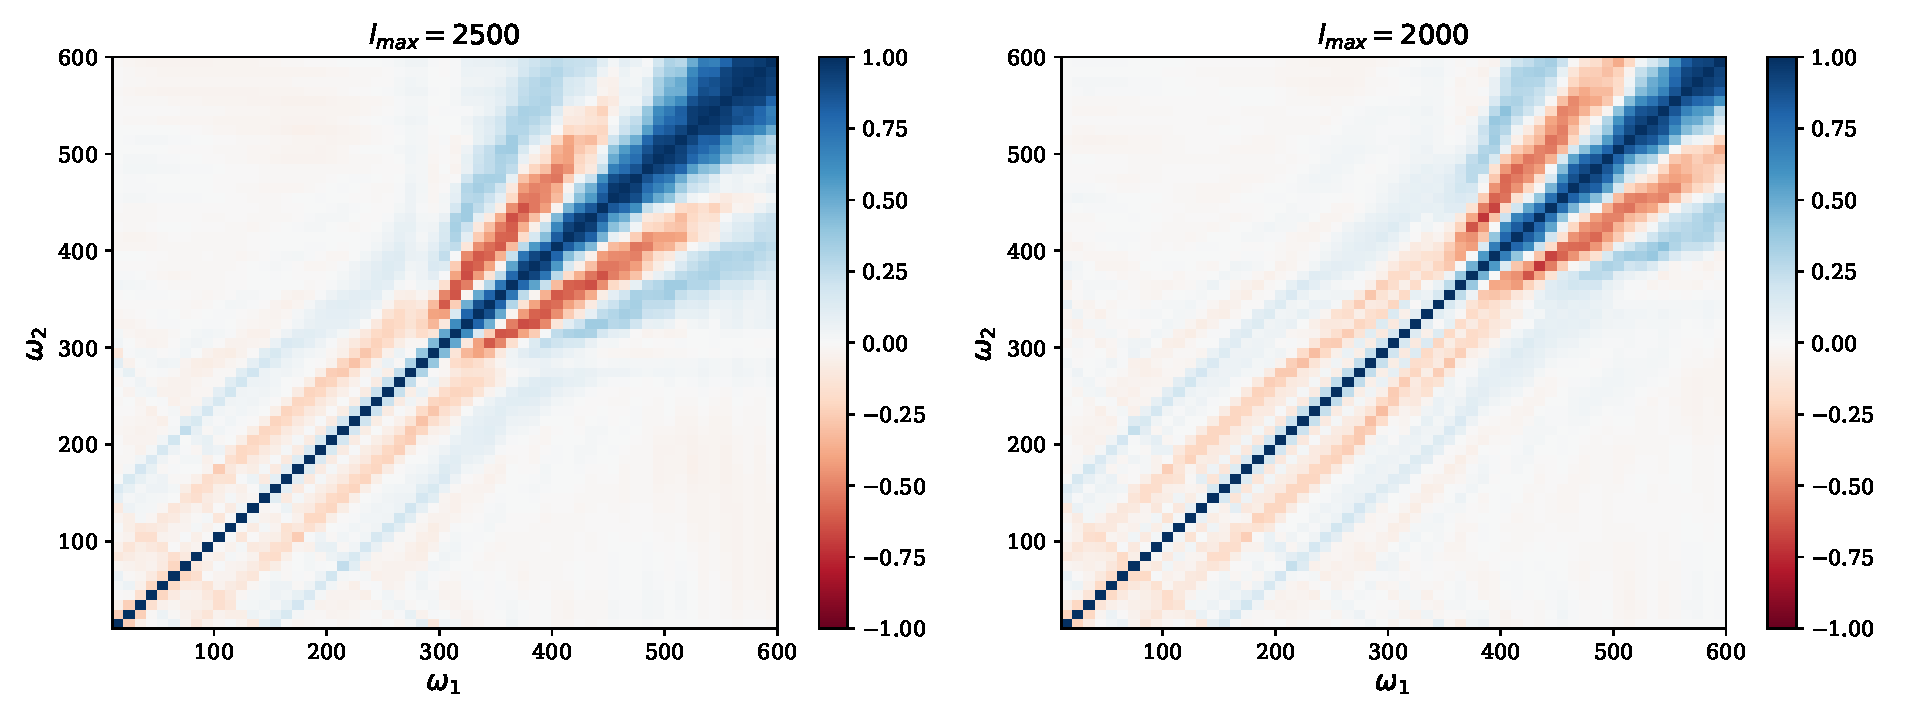
\includegraphics[width=\textwidth]{sine_template_correlations_compare_lmax_new.pdf}
	\caption{Theoretical correlations between feature model templates with different frequency $\omega$s, as described in Figure \ref{fig:feature_template_correlations}. The phase $\phi$ is set to zero in both cases, while the right plot is obtained from Legendre basis with a different $k$ range. The maximum $l$ value is reduced from $2500$ to $2000$, shifting $(k_{min},k_{max})$ by a factor of $2000/2500 = 0.75$. Having smaller $k$ range means fewer oscillations within the $k$ interval for same $\omega$, which provides better effective resolution. The right plot does indeed show smaller non-diagonal correlations at high frequencies.}
	\label{fig:feature_template_correlations_compare_lmax}
\end{figure}

There is one subtlety about $f_{NL}$ estimates obtained from inaccurate primordial basis expansions. CMB-BEst computes $\beta$s and $\Gamma$s with respect to the fixed Legendre basis, which has been shown to be accurate even for the highest degree of polynomials. When the primordial basis is unable to resolve rapid modulations as we have seen, the $f_{NL}$ estimates we obtain are nevertheless meaningful; they are simply probing the wrong model. The constraints are not for the given shape function, but rather its projection to the vector subspace spanned by the basis functions as shown in (\ref{eqn:primordial_basis_projection}). Detecting non-zero $f_{NL}$ here is can still have significant implications.

Another popular template for models with oscillations is the `resonance' shape parametrised as $S(k_1, k_2, k_3) = \sin(\omega \log(k_1 + k_2 + k_3 ) + \phi)$. Log-spaced modulations are numerically harder to deal with since the oscillation frequency diverges as $k \rightarrow 0$. Note also that any scaling factors to the $k$'s can be absorbed into the phase via $\log(c(k_1 + k_2 + k_3)) = \log(k_1 + k_2 + k_3) + \log(c)$. For our Legendre basis with $k_{max}/k_{min}$ fixed to $1000$, the full $k$ range includes $\approx 1.1\omega$ oscillations. Any frequency larger than $\approx 27$ therefore cannot be expanded using $p_{max}=30$ polynomials. We still explore shapes with higher $\omega$s however, since the basis can pick up slower oscillations in higher $k$ values. Corresponding constraints should be taken with a grain of salt; they probe bispectrum shapes \textit{similar} to the resonance template. Low-$k$ oscillations are especially likely to be wiped out from these shapes.

Figure \ref{fig:sinlog_template_frequency_Legendre_Modal} compares $f_{NL}$ constraints for the resonance template over a range of $\omega$s. As can be seen from the top two plots, the signal-to-noise values obtained from Legendre basis and Modal are relatively consistent up until $\omega \approx 35$, after which the two results start diverging significantly. The threshold is about the same for `sinlog' ($\phi = 0$) and `coslog' ($\phi=\pi/2$) shapes.

Recall that the sample $\sigma$ from $f_{NL}$ estimates of Gaussian simulations should converge to the theoretical value calculated from Fisher information as $N_{sims}\rightarrow\infty$, since the CMB bispectrum estimator is optimal. We have checked that the sample and theoretical variances are consistent for standard templates in Section \ref{section:internal_consistency}, using both KSW and Legendre basis sets. The bottom two plots in Figure \ref{fig:sine_template_frequency_Legendre_Modal} show the equivalent results for resonance template with varying $\omega$.

\begin{figure}[htbp!] 
	\centering    
	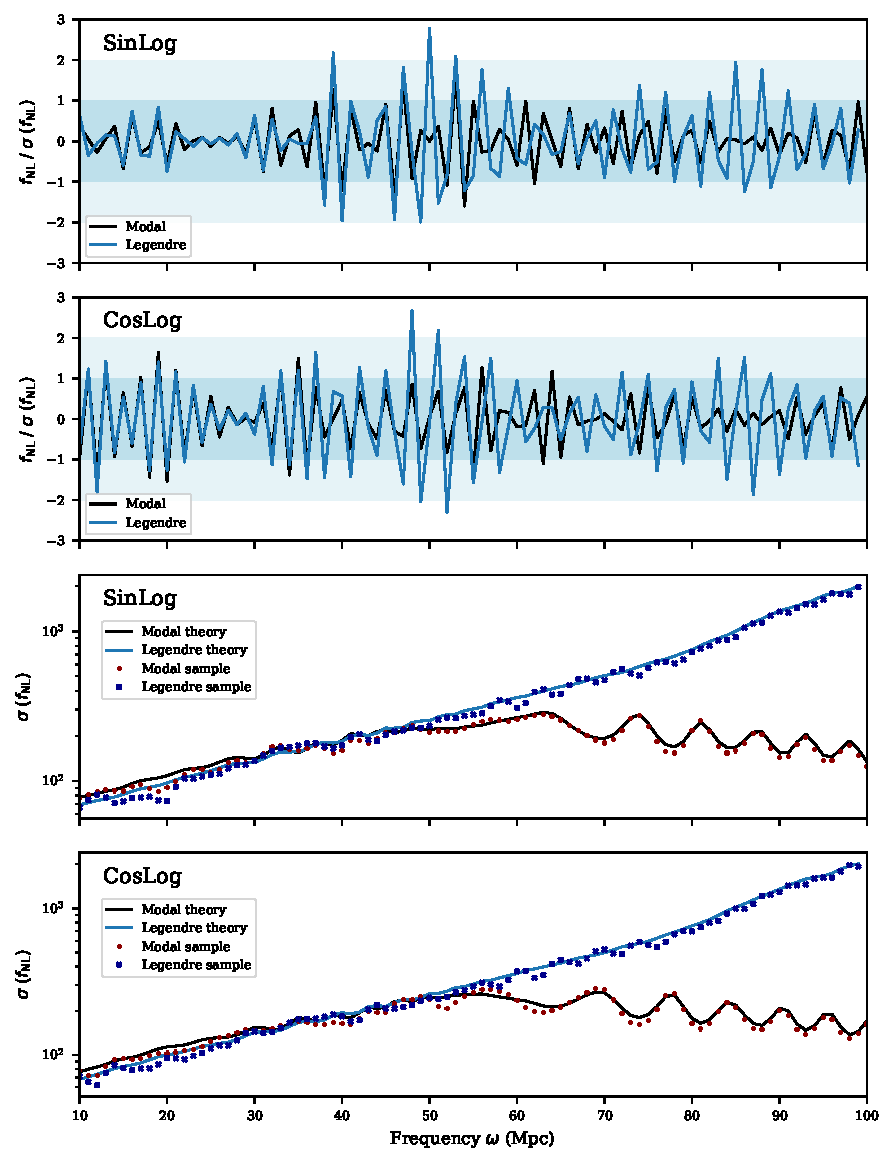
\includegraphics[width=\textwidth]{sinlog_template_frequency_Legendre_Modal.pdf}
	\caption{Constraints for the resonance shape $S(k_1,k_2,k_3) = \sin(\omega \log(k_1 + k_2 + k_3 ) + \phi)$ with varying $\omega$s and $\phi$ set to $0$ (left) and $\pi/2$ (right). Results are obtained using CMB-BEst's Legendre basis (blue) and Planck's Modal estimator (black). Top: signal-to-noise significance of the estimated $f_{NL}$s with $1\sigma$ and $2\sigma$ levels shaded in blue. Bottom: standard deviations of the $f_{NL}$ estimates against frequency $\omega$, calculated from the $f_{NL}$s of 140 simulations (sample) and the $\Gamma$ matrix (theory).}
	\label{fig:sinlog_template_frequency_Legendre_Modal}
\end{figure}

Similarly to the feature models studied in Chapter \ref{chapter:CMB_state-4_forecast}, uncertainty in the estimated $f_{NL}$s increases as we raise $\omega$, exploring more rapid oscillations in bispectrum. Both Modal and Legendre methods lose their ability to resolve shapes with $\omega$s larger than $35$. The constraints are then no longer for the precise resonance shape but rather an approximation to it. A notable difference between Modal and CMB-BEst's Legendre basis is their behaviour at high $\omega$. Modal's numerical accuracy is completely lost after $\omega\approx 50$, leading to disproportionately large bispectra and small $\sigma$. On the other hand, Legendre retains stability in its basis expansion, yielding constraints for approximate bispectrum shapes closest to the true, high-frequency ones.

\begin{figure}[htbp!] 
	\centering    
	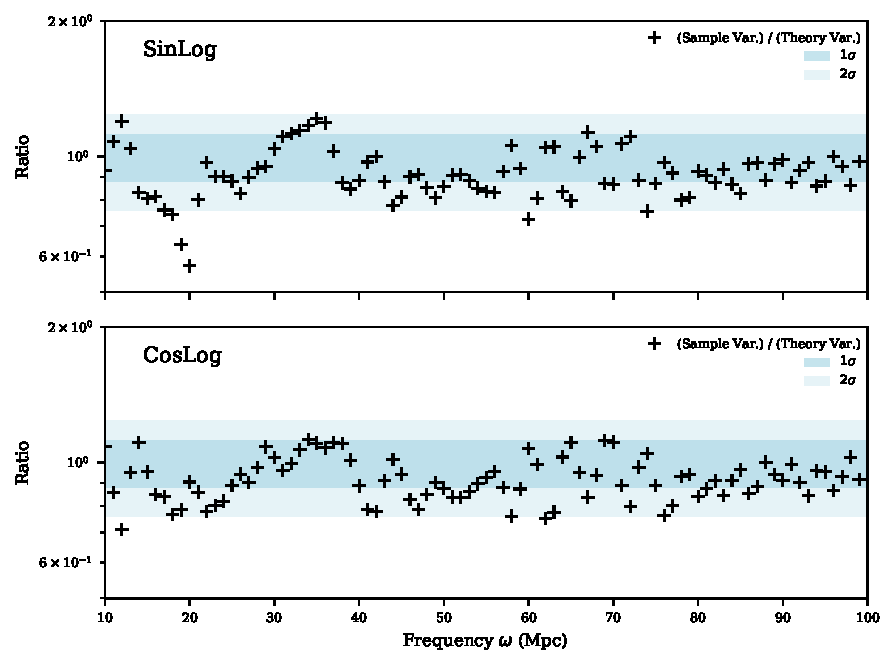
\includegraphics[width=\textwidth]{sinlog_template_frequency_variances_Legendre.pdf}
	\caption{Ratio between sample and theoretical variances obtained from Legendre basis for resonance shapes. Sampled variance is calculated from $f_{NL}$ estimates of $140$ Gaussian simulations. $1\sigma$ and $2\sigma$ intervals are chosen based on a $\chi^2$-distribution, which accurately describes sample variances as long as the $f_{NL}$s are normally distributed. Results are statistically consistent with random fluctuations except potentially one at $\omega=20$, discussed in the main text.}
	\label{fig:sinlog_template_frequency_variances_Legendre}
\end{figure}

A detailed comparison between the sample and theoretical variances is depicted in Figure \ref{fig:sinlog_template_frequency_variances_Legendre}. This serves as a useful consistency check within the CMB-BEst pipeline. Sample variances are calculated from finite number of $f_{NL}$ samples from simulations. We test if these estimates are compatible with the underlying distribution: $\chi^2$ with $N_{sims}-1$ degrees of freedom in this case. We achieve the desired consistency for both $\phi=0$ and $\phi=\pi/2$. One potentially meaningful outlier is at $\omega=20$ and $\phi=0$, where the sample estimate is below 60\% of the expected level. This anomaly is not likely to be a numerical error specific to CMB-BEst since a similar dip can be found from Modal results in Figure \ref{fig:sinlog_template_frequency_Legendre_Modal}. No significant irregularity is found for different phases at the same frequency. We classify this point as a random fluctuation for now, but a further investigation using an independent set of Gaussian simulations is required to be certain.

As with the feature models before, we plot the correlation matrix between the templates with different $\omega$s in Figure \ref{fig:sinlog_template_correlations}. Shapes with similar $\omega$s are naturally correlated, but most off-diagonal terms of the matrix vanish. Even for $\omega > 35$ where the basis expansion become less accurate, cross-correlations tend to remain small until $\omega \approx 75$. We verify the stability of CMB-BEst's Legendre basis expansion; best approximations to the highly oscillatory template is found, allowing us to continue exploring independent bispectrum shapes with the characteristic log-spaced oscillations.

\begin{figure}[htbp!] 
	\centering
	(a) $ \phi=0 $
	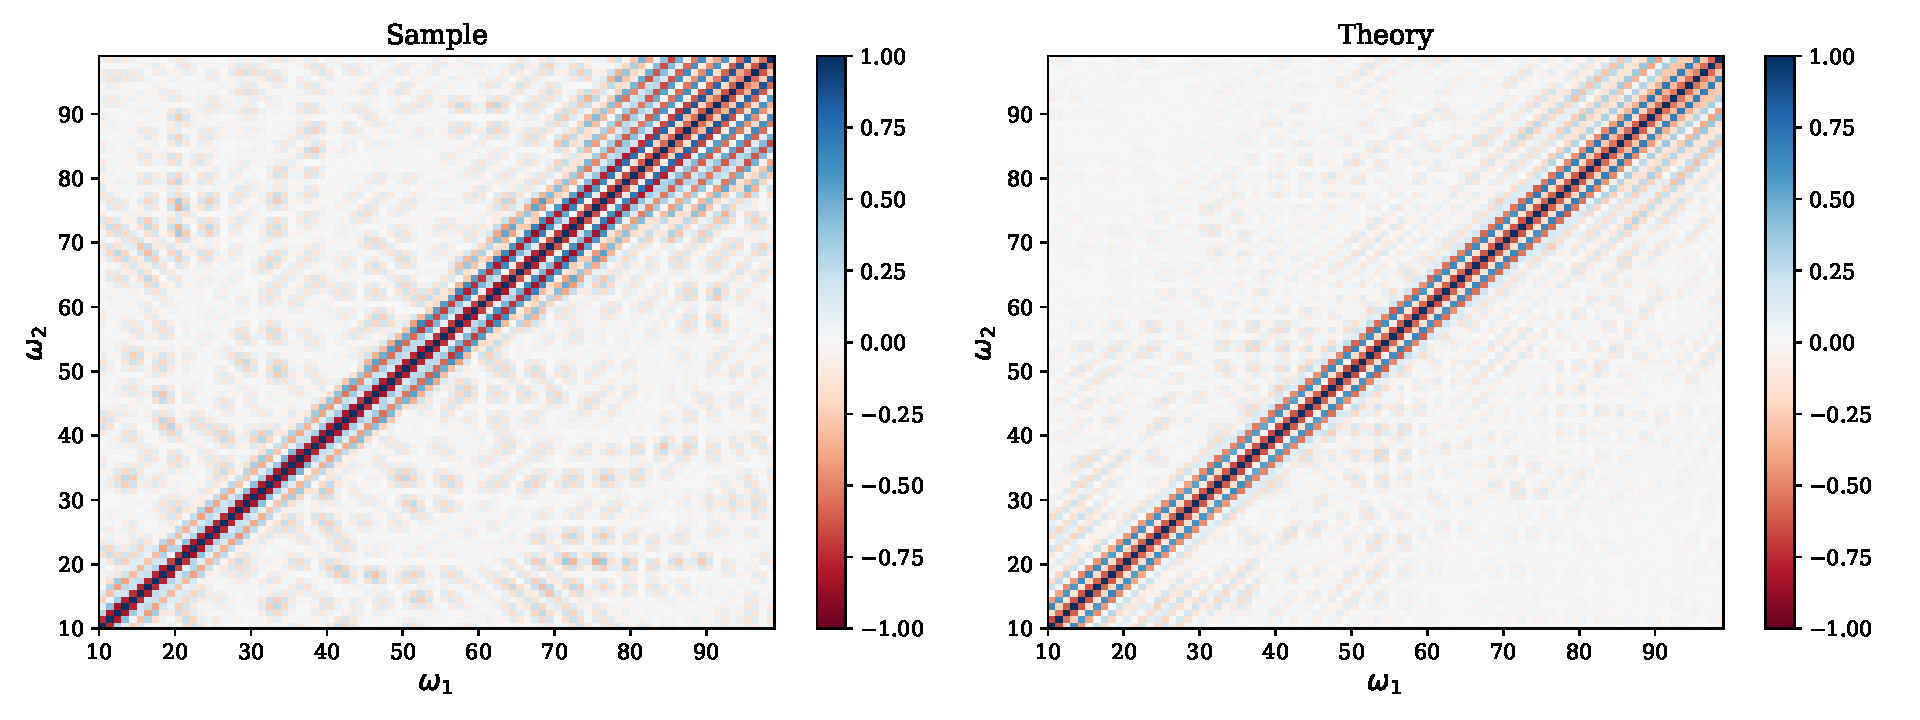
\includegraphics[width=\textwidth]{sinlog_template_correlations_new.pdf}
	(b) $ \phi=\pi/2 $
	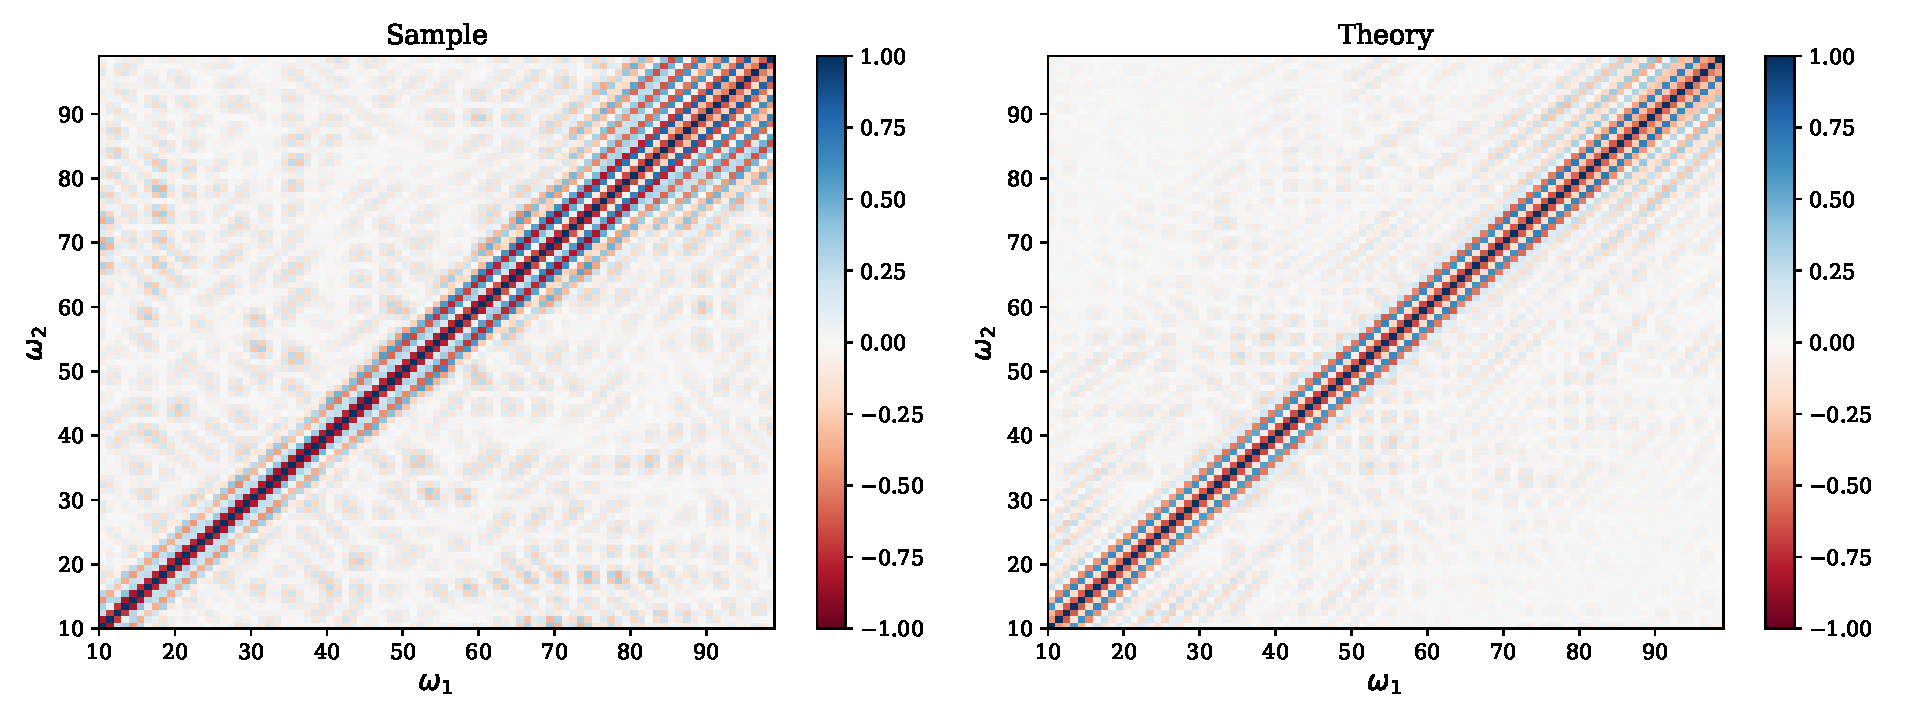
\includegraphics[width=\textwidth]{coslog_template_correlations_new.pdf}
	\caption{Correlations between resonance model templates $S(k_1,k_2,k_3) = \sin(\omega\log(k_1+k_2+k_3)+\phi)$ with different $\omega$ values, for (a) $\phi = 0$ and (b) $\phi=\pi/2$. `Sample' correlations are obtained from the Legendre basis $f_{NL}$ estimates from 140 Gaussian simulations. `Theory' correlations come from the inner product induced by $\Gamma$ matrix as shown in (\ref{eqn:late_time_inner_product}).}
	\label{fig:sinlog_template_correlations}
\end{figure}


\subsection{Proof of concept} \label{section:proof_of_concept}


\textsc{Primodal} is an efficient numerical code for computing bispectra of primordial perturbations using the in-in formalism \cite{Clarke2021}. Unlike many in-in codes, the computed bispectrum is expressed as coefficients of a separable basis expansion as opposed to a grid of discrete points. Choosing an equivalent basis set for \textit{CMB-BEst} therefore allows a direct link between the two codes. The combined pipeline is capable of constraining specific inflation models directly without the use of approximate templates. Such template-free bispectrum analysis also enables a fast and extensive scan of theory parameters.

Collaborating closely with the main author of \textsc{Primodal}, Philip Clarke, we verified the integrity of the combined \textsc{Primodal} + CMB-BEst routine. We thoroughly tested the consistency of basis functions, their orthogonalisation, and convergence. Both \textsc{Primodal} and \textsc{CMB-BEst} are now in the exploitation phase. We present a working example of the combined pipeline as a proof of concept.

DBI inflation \cite{Silverstein2004dbi,Alishahiha2004dbi} (TODO: add more DBI paper references) is a well-studied single-field inflation model inspired by string theory. Its action follows the general form \eqref{eqn:general_single_field_action}, with a non-canonical kinetic term given by
\begin{align}
	P(X,\phi) = - \frac{1}{f(\phi)} \left[ \sqrt{1 - 2f(\phi)X} - 1 \right] - V(\phi),
\end{align}
where $X=-\frac{1}{2} g^{\mu\nu} \partial_\mu \phi \partial_\nu \phi$ as before. $f(\phi)$ is an arbitrary function called the warp factor. We choose
\begin{align}
	f(\phi) = \frac{\lambda_{DBI}}{\phi^4}, \qquad V(\phi) = V_0 - \frac{1}{2}m^2\phi^2, \qquad m = \sqrt{\beta_{IR}} \; H
\end{align}

- DBI sound speed constraints
- DBI resonance scan
- tetrapyd decomp? 

\begin{figure}[htbp!] 
	\centering    
	\includegraphics[width=\textwidth]{dbi_sound_speed_scan_annotated_new.pdf}
	\caption{Constraints on the DBI model with varying sound speed $c_s$. Primordial bispectrum computed from \textsc{Primodal} is fed directly into CMB-BEst as coefficients $\alpha_{p_1 p_2 p_3}$ appearing in the Legendre basis expansion. Constraints from the Legendre basis with $p_{max}=30$ (black) are shown in comparison with $p_{max}=29$ (blue). $1\sigma$ and $2\sigma$ confidence intervals around $0$ are shaded in blue and represent the uncertainty in estimated $f_{NL}$s. Bispectrum shapes are normalised so that $f_{NL}=1$ corresponds to the DBI model in consideration. Our constraints on DBI sound speed is $c_s > 0.056$ with $95\%$ confidence.}
	\label{fig:dbi_sound_speed_scan}
\end{figure}

\begin{figure}[htbp!] 
	\centering    
	\includegraphics[width=0.8\textwidth]{dbi_reso_scan_fNLs_new.pdf}
	\caption{Constraints on the DBI model with oscillations imposed on the inflationary potential, causing resonance-type bispectra approximately parametrised as $\sin(\omega \log(k_1+k_2+k_3) + \phi)$. Primordial bispectrum is computed from \textsc{Primodal} for various step sizes, which was then are fed directly to CMB-BEst.}
	\label{fig:dbi_resonance_scan}
\end{figure}

\begin{figure}[htbp!] 
	\centering    
	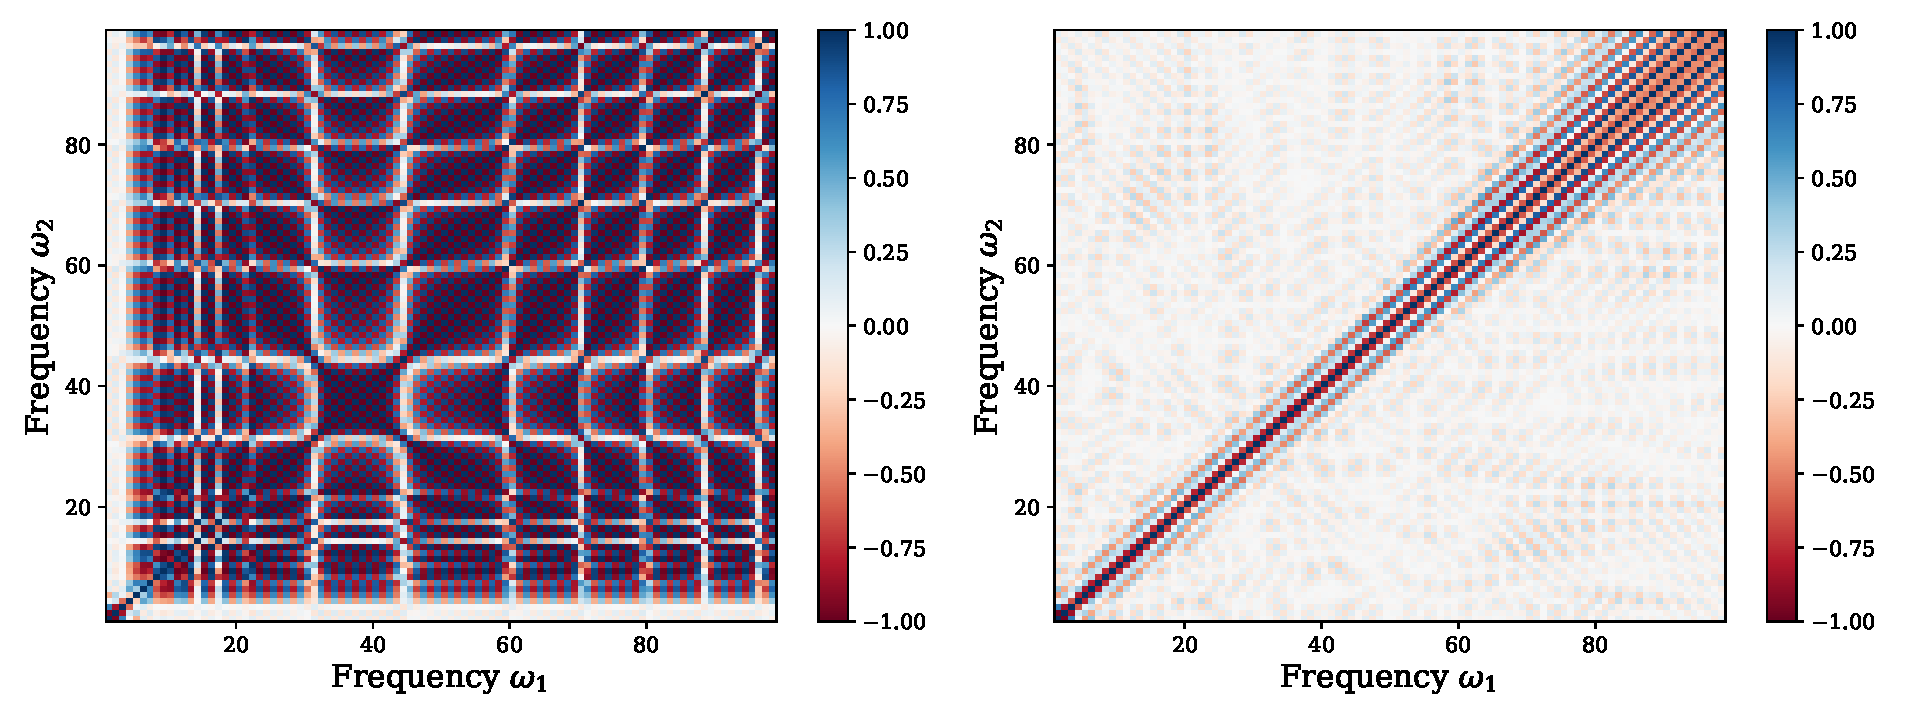
\includegraphics[width=\textwidth]{sinlog_equil_template_correlations_compare_decomp.pdf}
	\caption{Correlations between $f_{NL}$ constraints for the enveloped resonance shape $S(k_1,k_2,k_3) = S^{equil}(k_1,k_2,k_3) \sin(\omega \log(k_1+k_2+k_3))$ with different $\omega$s. Since the given shape behaves badly in a region outside the tetrapyd but within the cubic domain of (\ref{eqn:basis_expansion}), we observe large off-diagonal correlations in the original Legendre basis expansion (Left). Manually setting the shape function to zero at these unphysical configurations therefore dramatically improves the numerical performance (Right). }
	\label{fig:sinlog_equil_template_decomp_comparison}
\end{figure}




\subsection{Future work}





% Old table
%\begin{table}[h]
%	\caption{Constraints for the standard templates for the KSW and Legendre basis from CMB-BEst, in comparison with the `Modal' pipeline from Planck 2018 analysis \cite{PlanckCollaboration2018}}
%	\centering
%	\label{table:trio_fNL_comparison_with_planck}
%	\renewcommand{\arraystretch}{1.5} 
%	\begin{tabular}{llrrr}
%		\toprule
%		Template & Estimator &  $f_{NL}^T$ &  $\bar{\sigma}^T$ &  $\sigma^T$ \\
%		\toprule
%		
%		Local & KSW &   -2.2 &      5.5 &      5.3 \\
%		& Legendre &   -2.0 &      5.9 &      5.7 \\
%		& Modal &   -0.6 &      6.4 &      6.1 \\
%		
%		\midrule
%		Equilateral & KSW &   16.7 &     61.1 &     67.7 \\
%		& Legendre &   15.2 &     61.7 &     67.7 \\
%		& Modal &   33.8 &     66.5 &     72.4 \\
%		
%		\midrule
%		Orthogonal & KSW &   -6.9 &     37.6 &     33.7 \\
%		& Legendre &   -8.5 &     38.0 &     33.9 \\
%		& Modal &  -26.5 &     42.8 &     39.3 \\
%		\bottomrule
%	\end{tabular}
%\end{table}
